% \section{Analyzing Nonlinear Effects on 16-QAM WDM Signal Constellation Points Post-Compensation}

% \subsection{Abstract}
% In optical communication systems, the rigorous analysis of signal behavior post-compensation for chromatic dispersion and phase equalization is crucial for optimizing performance. This investigation delves into the analysis of 16-QAM Wavelength Division Multiplexing (WDM) signal constellation points post-compensation, revealing complex structural characteristics indicative of nonlinear effects within the channel.

\section{Introduction}
Optical communication channels often exhibit nonlinear effects that can significantly impact the integrity and recoverability of transmitted signals. Understanding of these effects is essential for designing robust communication systems capable of maintaining high levels of performance. 
With a deterministic model such as the \Gls{nlse} that closely corresponds with real systems, we can study this behavior in depth. If we consider that we have precise knowledge of the final distribution of constellation points at the receiver for any given input at the transmitter, we can leverage this information to our advantage. As new symbols arrive at the receiver, we might initially be uncertain about their identity. However, with comprehensive knowledge about the ultimate distribution of all constellation points, we can ascertain how likely it is that a new point corresponds to a specific symbol. This approach allows us to accurately map each new point to the correct constellation symbol, enhancing the accuracy of the signal interpretation.

In pursuit of a deeper understanding of these effects, we turn to computational simulations. Specifically, we use a \acrshort{gpu}-based simulation package, HpCom~\cite{esf0_2023_7880552}, which allows us to generate a large amount of data. By analyzing the internal structure of the received constellation points, we aim to demonstrate that the nonlinear effects induce distinctive patterns in the data. These patterns are not merely noise; they hold valuable information about the behavior of the signal within the fiber. Through detailed analysis, we can begin to reveal these patterns and improve our ability to predict and mitigate the impact of nonlinearity on our communications, pushing the boundaries of what's possible in optical data transmission. 

In this study of optical communication systems, we initially ignore \acrfull{ase} noise to focus on how signals change due to nonlinear effects alone. This choice is not by mistake but a planned decision to look closely at how nonlinear effects work together without noise interference. By considering signal changes as a predictable process due to nonlinear effects, we can better understand these effects without the randomness of noise getting in the way.

We know this approach has its downsides. It's important to point out that leaving out noise is a first step in our analysis. Our goal is to clearly see how pure nonlinear effects shape the signals we receive. This makes our analysis simpler and helps us get to the basics of how nonlinear effects influence signal changes. This basic understanding is crucial for coming up with new ideas and algorithms to handle these nonlinearities better.
Yet, we accept that this simplification is just the beginning. The way noise and nonlinear effects interact is important for a complete picture of optical systems, but this thesis does not cover that.

To sum up, this thesis looks at the predictable nonlinear effects in optical communication systems. Future studies will build on this work to also include how noise affects these systems.


\section{Methodology}

\begin{figure}[htpb]
    \center{
        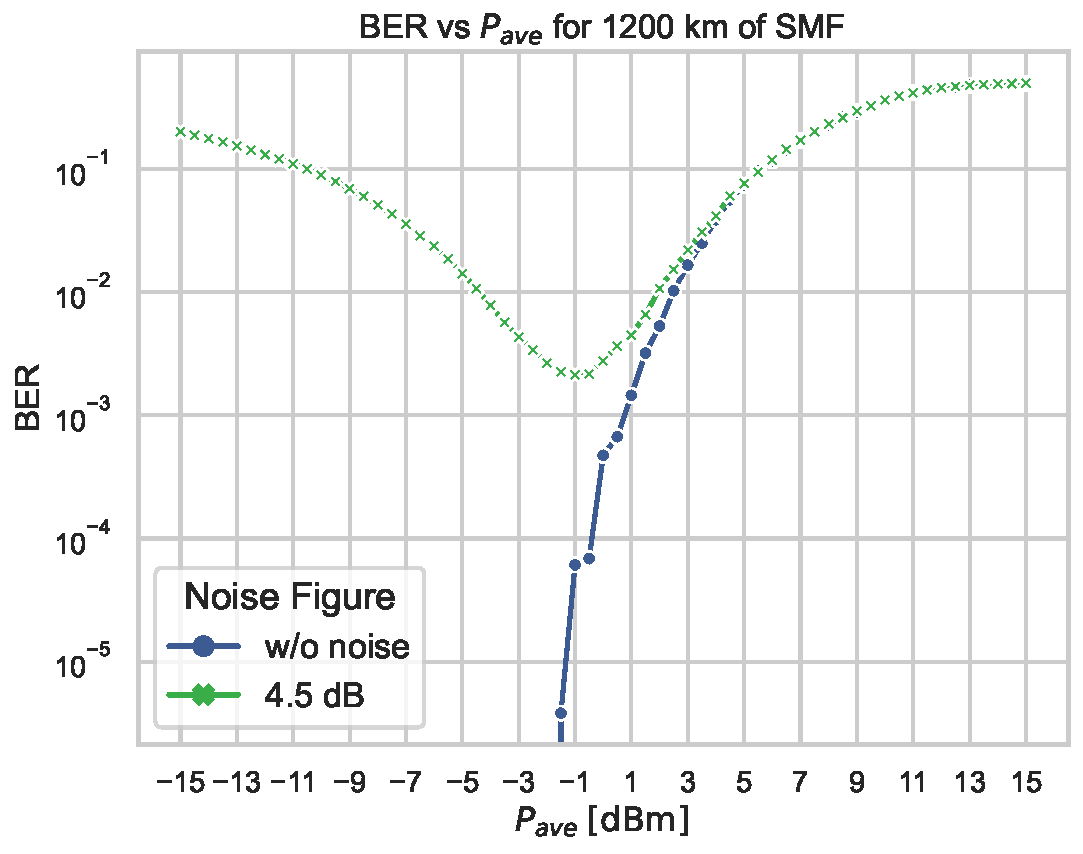
\includegraphics[width=0.7\linewidth]{images/benchmark/ber_vs_p_ave_dbm_z1200.pdf} \\
    }
    \caption{BER vs $P_{ave}$ \textrm{[dBm]} for studied system. The green line marked with crosses represents the reference system, including the impact of additional \acrshort{edfa} noise characterized by a 4.5 dB Noise Figure. The blue line illustrates the ideal case, free from \acrshort{ase} noise, which is the focus of our study.
    }
    \label{fig:ber_vs_pave_z1200}
\end{figure}

This study focuses on the analysis of a 16-\acrshort{qam} \acrshort{wdm} signal, specifically investigating the behavior of received constellation points post-\Gls{cdc} and \Gls{npe}.
We employed an optical channel model of \acrfull{ssmf} with \acrlong{edfa}s (\acrshort{edfa}s). The signal format under consideration is a 16-\acrshort{qam} \acrshort{wdm} with single polarization and a symbol rate of \(34.4\; \text{GBd}\). Pulse shaping was realized using a digital \acrfull{rrc} filter with a roll-off factor of \(0.1\). The total transmission distance spanned \(15\) links of \(80\; \text{km}\) each. The \acrshort{edfa} was assumed to be ideal, introducing no noise. The average signal power varied from \(-2\) to \(8\; \text{dBm}\).
Signal propagation through the fiber was modeled by the nonlinear Schrödinger equation (NLSE), which was solved using the \acrshort{gpu}-accelerated split-step Fourier method\cite{esf0_2023_7880552}. The fiber's parameters were set to a wavelength of \(\lambda = 1550\; \text{nm}\), a dispersion coefficient of \(D = 16.8\; \text{ps/nm}\cdot\text{km}\), and a nonlinear coefficient of \(\gamma = 1.2\; \text{W}^{-1}\cdot\text{km}^{-1}\).
For the study, we generated \(2^{24}\) data points for each specified average power level.

Figure~\ref{fig:ber_vs_pave_z1200} illustrates the dependence of the \gls{ber} on the average signal power for the system parameters described previously. It depicts two scenarios: one with additional noise from \gls{edfa} and one without. The power range under investigation is selected to align with the optimal levels for real-world transmission systems. As indicated by the graph (represented by the green line), the \gls{ber} reaches its minimum around \(-1\) dBm. It is important to note that, for the purposes of our study, we utilize data from the channel without \gls{edfa} noise. This approach allows us to specifically examine the impact of nonlinearity without the confounding effects of random noise.


\begin{figure}[h]
    \center{
        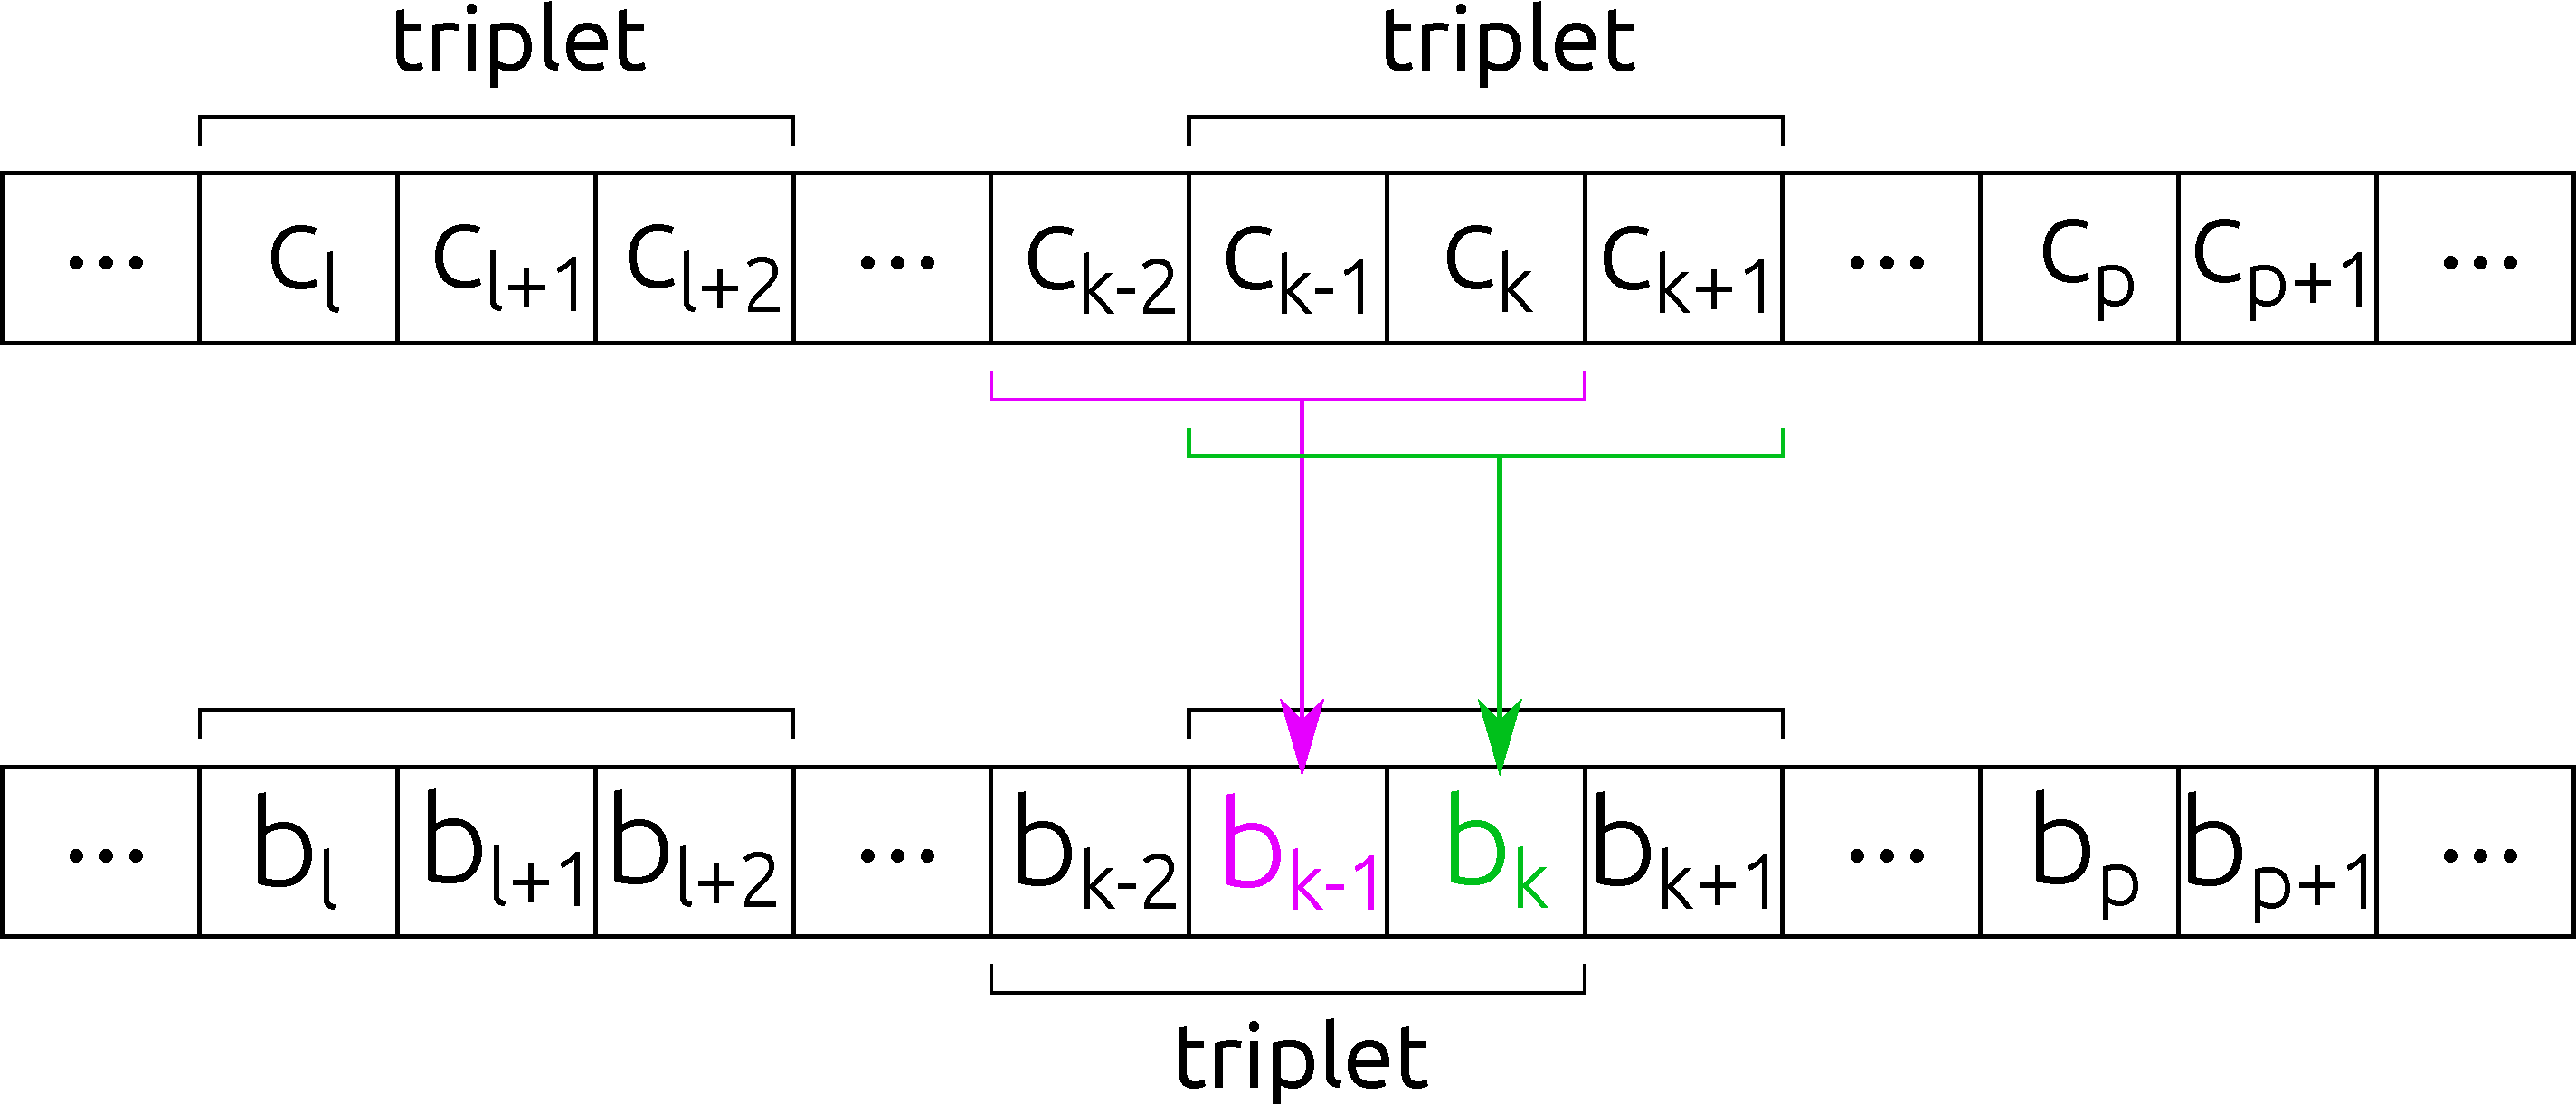
\includegraphics[width=1\linewidth]{images/gauss/triplets.pdf}
    }
    \caption{Schematic representation of the ``triplet'' concept, illustrating the extraction of data \( b_k \) corresponding to each transmitted triplet \( (c_{k-1}, c_k, c_{k+1}) \).
}
    \label{fig:triplet}
\end{figure}

In this work, we introduce the concept of a ``triplet'', which is defined as a set of three consecutive points consisting of a left, central, and right point (Fig.~\ref{fig:triplet}). On the transmitter side, there is a sequence of transmitted symbols. Unlike real systems where the sequence is continuous and lacks a definitive beginning or end, our simulation employs a cyclic version: \(\{c_0, c_1, \ldots, c_{k-1}, c_k, c_{k+1}, \ldots, c_{K-1}, c_{K}\}\), where \(K\) represents the total number of transmitted symbols. In the continuum of transmitted constellation symbols \(c_k\), a triplet is any set of three points \((c_{k-1}, c_k, c_{k+1})\) for the transmitted sequence. Similarly, for received symbols \(b_k\), we define a triplet as \((b_{k-1}, b_k, b_{k+1})\). Our focus is on the distributions of the received symbol \(b_k\) for a specific transmitted triplet \((c_{k-1}, c_k, c_{k+1})\). In essence, we aim to categorize our dataset and analyze the distributions for \(b_k\) based on the transmitted symbol and its adjacent neighbors.

% Within the dataset, we can isolate all points \(b_k\) corresponding to any particular transmitted triplet \((c_{k-1}, c_k, c_{k+1})\). For a 16-\Gls{qam} system, there exist \(16 \times 16 \times 16 = 2^{12}\) potential triplet combinations. With \(2^{24}\) data points in our dataset, this results in approximately \(2^{12}\) data points per triplet, available for further analysis.

\begin{figure}[h]
    \center{
        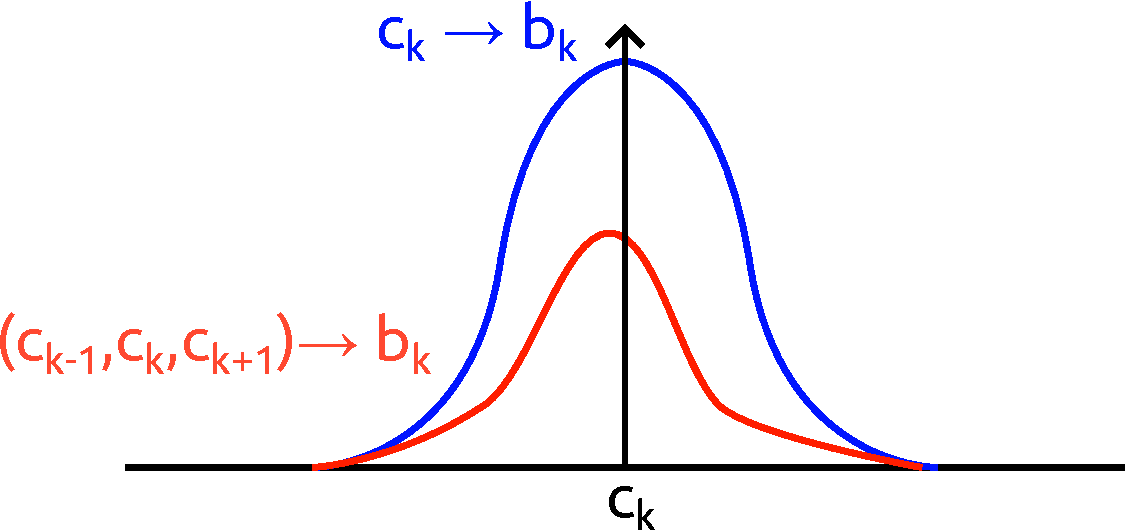
\includegraphics[width=0.6\linewidth]{images/gauss/distribution.pdf}
    }
    \caption{Schematic illustration of received symbol distributions based on transmitted triplets. The blue line represents the distribution of received symbols $b_k$ originating from the transmission of a single symbol $c_k$. The red line shows the modified distribution of $b_k$ when considering the entire transmitted triplet $(c_{k-1}, c_k, c_{k+1})$.
    }
    \label{fig:triplet_distribution}
\end{figure}

In our simulation setup, we maintain a fixed average signal power for the transmitted signal (we conduct separate analyses for each signal power level, ranging from $-2$ dBm up to $8$ dBm). This setup provides us with complete information, including the sequence of transmitted symbols $\{c_k\}$ and the sequence of received symbols $\{b_k\}$. It is important to note that for this analysis, the received symbols $\{b_k\}$ have already been compensated for dispersion and phase shift, allowing us to concentrate solely on the deviations in the complex constellation plane caused by nonlinear interactions.

To analyze the impact of these nonlinear interactions, we examine the distributions of the received symbols $\{b_k\}$ based on their originating "triplet" $(c_{k-1}, c_k, c_{k+1})$. This process involves iteratively selecting indices $k$ corresponding to each specific triplet configuration (for example, $(c_{k-1}, c_k, c_{k+1})$ is $(1+1\mathrm{j}, 1+3\mathrm{j}, -3-1\mathrm{j})$ or any other triplet), and gathering all corresponding $b_k$. 
For a 16-\Gls{qam} system, there exist \(16 \times 16 \times 16 = 2^{12}\) potential triplet combinations. With \(2^{24}\) data points in our dataset, this results in approximately \(2^{12}\) data points per triplet, available for further analysis.Through this method, we create distributions of received symbols $D(b_{k})$ for each of the $2^{12}$ possible triplet combinations, thereby associating each distribution $D(b_{k})$ with its respective sent triplet $(c_{k-1}, c_k, c_{k+1})$.

To simplify the analysis, we normalize the distributions of $b_k$ for each triplet by subtracting the original transmission point $c_k$, shifting all distribution centers towards the origin $(0, 0)$. This adjustment aims to reduce the influence of the original transmission point's location on the analysis, allowing us to more clearly observe the shifts in distribution centers caused by nonlinear effects, which will be further explored in subsequent analysis steps.

Figure~\ref{fig:triplet_distribution} provides a schematic representation of this process: transmitting $c_k$ results in a distribution of received symbols $b_k$ (depicted by the blue line). When we limit the analysis to received symbols $b_k$ that correspond not only to the transmitted symbol $c_k$ but to the sent triplet $(c_{k-1}, c_k, c_{k+1})$, we observe a modified distribution (indicated by the red line).


The primary model utilized for distribution analysis is the \Gls{gmm}, which will facilitate the understanding of the underlying structure within the received signal constellations.

\subsection{Gaussian Mixture Model and Likelihood}

A \gls{gmm} is a probabilistic model that assumes all the data points are generated from a mixture of a finite number of Gaussian distributions with unknown parameters. The formula for a \acrshort{gmm} can be written as:
\begin{equation}
    p(\mathbf{x}) = \sum_{k=1}^K \pi_k \mathcal{N}(\mathbf{x} | \boldsymbol{\mu}_k, \boldsymbol{\Sigma}_k) {,}
    \label{eq:gmm}
\end{equation}
where \( \mathbf{x} \) is a data point, \( K \) is the number of Gaussian components, \( \pi_k \) is the mixing coefficient for the \(k\)th Gaussian component (with the constraint \( \sum_{k=1}^K \pi_k = 1 \)), \( \boldsymbol{\mu}_k \) is the mean vector of the \(k\)th Gaussian component, \( \boldsymbol{\Sigma}_k \) is the covariance matrix of the \(k\)th Gaussian component and 
\( \mathcal{N}(\mathbf{x} | \boldsymbol{\mu}_k, \boldsymbol{\Sigma}_k) \) is the Gaussian distribution.


In this study we will use likelihood function to compare different models for the same data. The model with the higher likelihood (or higher log-likelihood) is generally considered to have a better fit to the data.
For a given statistical model and observed data, the likelihood function $L(\theta|x)$ (where $\theta$ represents the parameters of the model and $x$ represents the observed data) quantifies how well the model with specific parameter values explains the data.

Let's consider a simple example for likelihood for single one-dimensional Gaussian distribution.
The likelihood function $L$ for a Gaussian distribution gives us a measure of how likely it is to observe a given set of data points $(x_1, x_2, \ldots, x_n)$ given the parameters of the Gaussian distribution, specifically the mean $\mu$ and variance $\sigma^2$.
For a set of independent and identically distributed observations from a Gaussian distribution, the likelihood function is:
% Likelihood function for a Gaussian distribution
\begin{equation}
    L(x_1, x_2, \ldots, x_n | \mu, \sigma^2) = \prod_{i=1}^{n} \frac{1}{\sqrt{2\pi\sigma^2}} \exp\left(-\frac{(x_i - \mu)^2}{2\sigma^2}\right)
\end{equation}

The log-likelihood is the natural logarithm of the likelihood function, which turns the product of probabilities into a sum of log probabilities, making it easier to work with especially for computations:
\begin{equation}
    \log L(x_1, x_2, \ldots, x_n | \mu, \sigma^2) = \sum_{i=1}^{n} \left[ -\frac{1}{2}\log(2\pi\sigma^2) -\frac{(x_i - \mu)^2}{2\sigma^2} \right]
\end{equation}
% Log-Likelihood function for a Gaussian distribution

If we return to two-dimensional case, for \gls{gmm} (Eq.~(\ref{eq:gmm})) the log-likelihood is given by:
\begin{equation}
\log p(\mathbf{X} | \boldsymbol{\pi}, \boldsymbol{\mu}, \boldsymbol{\Sigma}) = \sum_{n=1}^N \log \left( \sum_{k=1}^K \pi_k \mathcal{N}(\mathbf{x}_n | \boldsymbol{\mu}_k, \boldsymbol{\Sigma}_k) \right) {,}
\label{eq:loglik}
\end{equation}
where single two-dimensional datapoint $\mathbf{x_n} \in \mathbf{X}$ and \(k\) is the number of corresponding Gaussian component.

In our scenario, the two-dimensional data points $\mathbf{x}_n$ correspond to the received symbols $\{b_k\}$ associated with the selected triplet.

\subsection{Model fitting}

As previously discussed, within the dataset, we isolate all points \( b_k \) corresponding to any particular transmitted triplet \( (c_{k-1}, c_k, c_{k+1}) \). For each triplet in the 16-\Gls{qam} system, this results in approximately \( 2^{12} \) data points. Given the \( 2^{12} \) combinations of triplets, we conduct a comprehensive analysis in the following manner. Initially, we assign to each triplet a unique identifier (ID) for ease of representation. Several IDs that will be referenced in this text are listed in Table~\ref{tab:triplet_ids}:
\begin{table}[h]
    \caption{Triplet unique identifiers (IDs)}
    \begin{center}
        \begin{tabular}{cccc}
            \hline
            Left point & Central point & Right point & identifier (ID)\\ 
            \hline
            $1+3\mathrm{i}$ & $1+3\mathrm{i}$ & $3+1\mathrm{i}$ & 552 \\ %1+3j, 1+3j, 3+1j
            $-1-1\mathrm{i}$ & $1+1\mathrm{i}$ & $-1-1\mathrm{i}$ & 1285 \\ %-1-1j, 1+1j, -1-1j
            $3+3\mathrm{i}$ & $3+3\mathrm{i}$ & $3+3\mathrm{i}$ & 2730 \\ %3+3j, 3+3j, 3+3j
            $3-3\mathrm{i}$ & $3-3\mathrm{i}$ & $1-1\mathrm{i}$ & 2993 \\ %3-3j, 3-3j, 1-1j
            \hline
        \end{tabular}
    \label{tab:triplet_ids}
    \end{center}
\end{table} % ID 2730 $[3+3\mathrm{i}, 3+3\mathrm{i}, 3+3\mathrm{i}]$ and ID 1285 $[-1-1\mathrm{i}, 1+1\mathrm{i}, -1-1\mathrm{i}]$ ID 2993 $[3-3\mathrm{i}, 3-3\mathrm{i}, 1-1\mathrm{i}]$ and ID 552 $[1+3\mathrm{i}, 1+3\mathrm{i}, 3+1\mathrm{i}]$
For these triplets, we gather all corresponding points \( b_k \) and create a centered distribution $D(b_{k} - c_k)_{\mathrm{ID}}$ of \( b_k - c_k \). Although fitting the distribution is possible without this centering process, shifting the received points to align with the transmitted points simplifies the representation and interpretation of the data. Subsequently, we employ the BRMLtoolbox~\cite{barberBRML2012} to fit a \gls{gmm} distribution to the centered data. 


The \acrfull{em} algorithm is a powerful iterative method used to find the maximum likelihood estimates of parameters in statistical models, especially when the model depends on unobserved latent variables. In the context of \acrshort{gmm}s, the \acrshort{em} algorithm is used to estimate the parameters of the Gaussian distributions (means, variances, and mixture coefficients) that best fit the data.
The \acrshort{em} algorithm for \acrshort{gmm}s involves two main steps repeated iteratively: the Expectation step (E-step) and the Maximization step (M-step)~\cite{hastie2009elements,murphy2012machine}.

\subsubsection{E-Step}

In the E-step, the algorithm estimates the posterior probabilities that a given data point belongs to each of the Gaussian distributions. This is done using the current estimates of the parameters. These probabilities are known as ``responsibilities'' and are calculated based on Bayes' theorem.

Given \(K\) Gaussian distributions, the responsibility of the \(k\)-th distribution for the \(i\)-th data point, \(x_i\), is given by:

\[
\gamma(z_{ik}) = \frac{\pi_k \mathcal{N}(x_i | \mu_k, \Sigma_k)}{\sum_{j=1}^{K} \pi_j \mathcal{N}(x_i | \mu_j, \Sigma_j)}
\]

where:
\begin{itemize}
    \item \(\gamma(z_{ik})\) is the responsibility of the \(k\)-th Gaussian for \(x_i\),
    \item \(\pi_k\) is the mixture coefficient for the \(k\)-th Gaussian (the prior probability that a randomly chosen data point comes from the \(k\)-th Gaussian),
    \item \(\mathcal{N}(x_i | \mu_k, \Sigma_k)\) is the probability density of \(x_i\) under the \(k\)-th Gaussian distribution with mean \(\mu_k\) and covariance matrix \(\Sigma_k\).
\end{itemize}

\subsubsection{M-Step}

In the M-step, the algorithm updates the parameters of the Gaussian distributions (means, covariance matrices, and mixture coefficients) based on the responsibilities computed in the E-step. The updates are calculated to maximize the expected log-likelihood of the data.

The updated parameters are calculated as follows:

\begin{itemize}
    \item Updated mean for the \(k\)-th Gaussian:
    \[
    \mu_k^{new} = \frac{1}{N_k} \sum_{i=1}^{N} \gamma(z_{ik}) x_i
    \]
    
    \item Updated covariance matrix for the \(k\)-th Gaussian:
    \[
    \Sigma_k^{new} = \frac{1}{N_k} \sum_{i=1}^{N} \gamma(z_{ik}) (x_i - \mu_k^{new})(x_i - \mu_k^{new})^T
    \]
    
    \item Updated mixture coefficient for the \(k\)-th Gaussian:
    \[
    \pi_k^{new} = \frac{N_k}{N}
    \]
\end{itemize}

where \(N_k = \sum_{i=1}^{N} \gamma(z_{ik})\) is the effective number of data points assigned to the \(k\)-th Gaussian, and \(N\) is the total number of data points.

In the two-dimensional case, each data point \(x_i\) is a vector in \(\mathbb{R}^2\), and the covariance matrices \(\Sigma_k\) of the Gaussian distributions are \(2 \times 2\) matrices. The formulas for updating the means, covariance matrices, and mixture coefficients remain the same. However, the computation of the probability density \(\mathcal{N}(x_i | \mu_k, \Sigma_k)\) for each data point involves the two-dimensional Gaussian density function, which takes into account the covariance between the two dimensions for each Gaussian component.
This model allows for capturing more complex shapes in the data distribution by considering the correlations between dimensions, making \acrshort{gmm}s a powerful tool for clustering and density estimation in multivariate data.


The analysis includes fitting \gls{gmm} models with a number of Gaussian components ranging from one to five. For instance, a \gls{gmm} with two components yields the following properties from the fitting process:
\begin{enumerate}
    \item \textbf{Log-likelihood.} Log-likelihood of the data for the particular \gls{gmm} parameters. The log-likelihood is given by Eq.~(\ref{eq:loglik}).

    \item \textbf{Mixing coefficients.} \( \pi_1 \) and \( \pi_2 \) are the mixing coefficient for the first and second Gaussian components respectively (\( \pi_1 + \pi_2 = 1 \)).

    \item \textbf{Mean Vectors.} For the first and second Gaussian component:
    \[
    \boldsymbol{\mu}_1 = \begin{pmatrix} \mu_{1,1} \\ \mu_{2,1} \end{pmatrix} \quad \text{and} \quad 
    \boldsymbol{\mu}_2 = \begin{pmatrix} \mu_{1,2} \\ \mu_{2,2} \end{pmatrix} {.}
    \]
    
    \item \textbf{Covariance Matrices.} For the first and second Gaussian component:
    \[
    \boldsymbol{\Sigma}_1 = \begin{pmatrix} \sigma_{11,1} & \sigma_{12,1} \\ \sigma_{21,1} & \sigma_{22,1} \end{pmatrix}
    \quad \text{and} \quad
    \boldsymbol{\Sigma}_2 = \begin{pmatrix} \sigma_{11,2} & \sigma_{12,2} \\ \sigma_{21,2} & \sigma_{22,2} \end{pmatrix} {.}
    \]
    
    \item \textbf{Eigenvalues.} The eigenvalues of the covariance matrices could be obtained by solving the characteristic equation \(\text{det}(\boldsymbol{\Sigma} - \lambda \boldsymbol{I}) = 0\), where \(\boldsymbol{I}\) is the identity matrix. For the first and second Gaussian components, the eigenvalues could be represented as follows:
    \[
    \boldsymbol{\lambda}_1 = \begin{pmatrix} \lambda_{1,1} \\ \lambda_{2,1} \end{pmatrix} \quad \text{and} \quad 
    \boldsymbol{\lambda}_2 = \begin{pmatrix} \lambda_{1,2} \\ \lambda_{2,2} \end{pmatrix} {.}
    \]
\end{enumerate}

For other numbers of Gaussian components, the data is processed in a similar manner. All fitting results are stored for further analysis and are accessible from my GitHub repository or via email. Detailed information and data sets can be obtained through the following repository link or by contacting me directly\footnote{GitHub Repository: \href{https://github.com/esf0}{https://github.com/esf0}. Email: \href{mailto:egor.sedoff@gmail.com}{egor.sedoff@gmail.com}}. In the subsequent section, specific results and insights gleaned from the data will be presented.


\section{Results}

\begin{figure}[hp]
    \begin{minipage}[h]{0.33\linewidth}
    \center{
        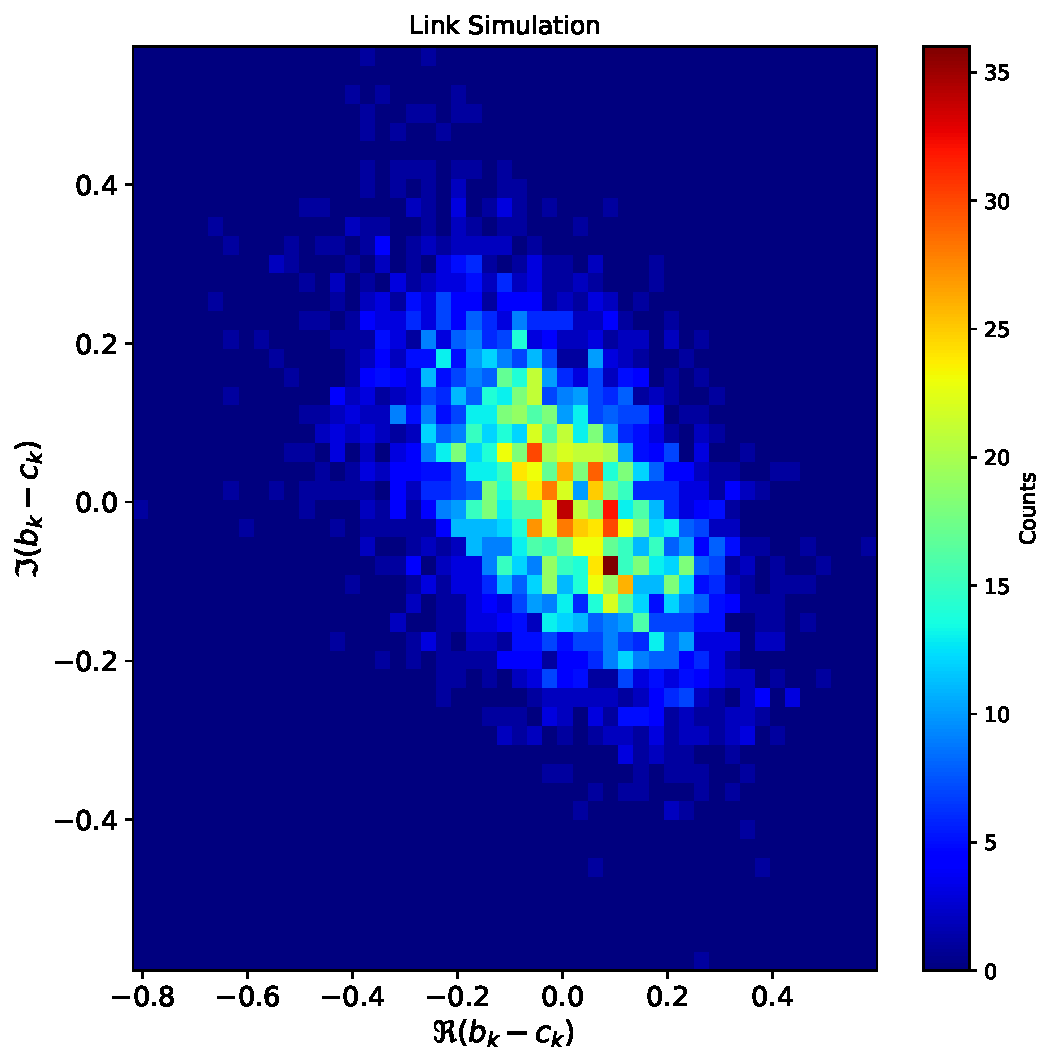
\includegraphics[width=1\linewidth]{images/gauss/exp_fit_triplet_552_dir1_pavedbm-2.pdf} \\
    }
    \end{minipage}
    \begin{minipage}[h]{0.33\linewidth}
    \center{
        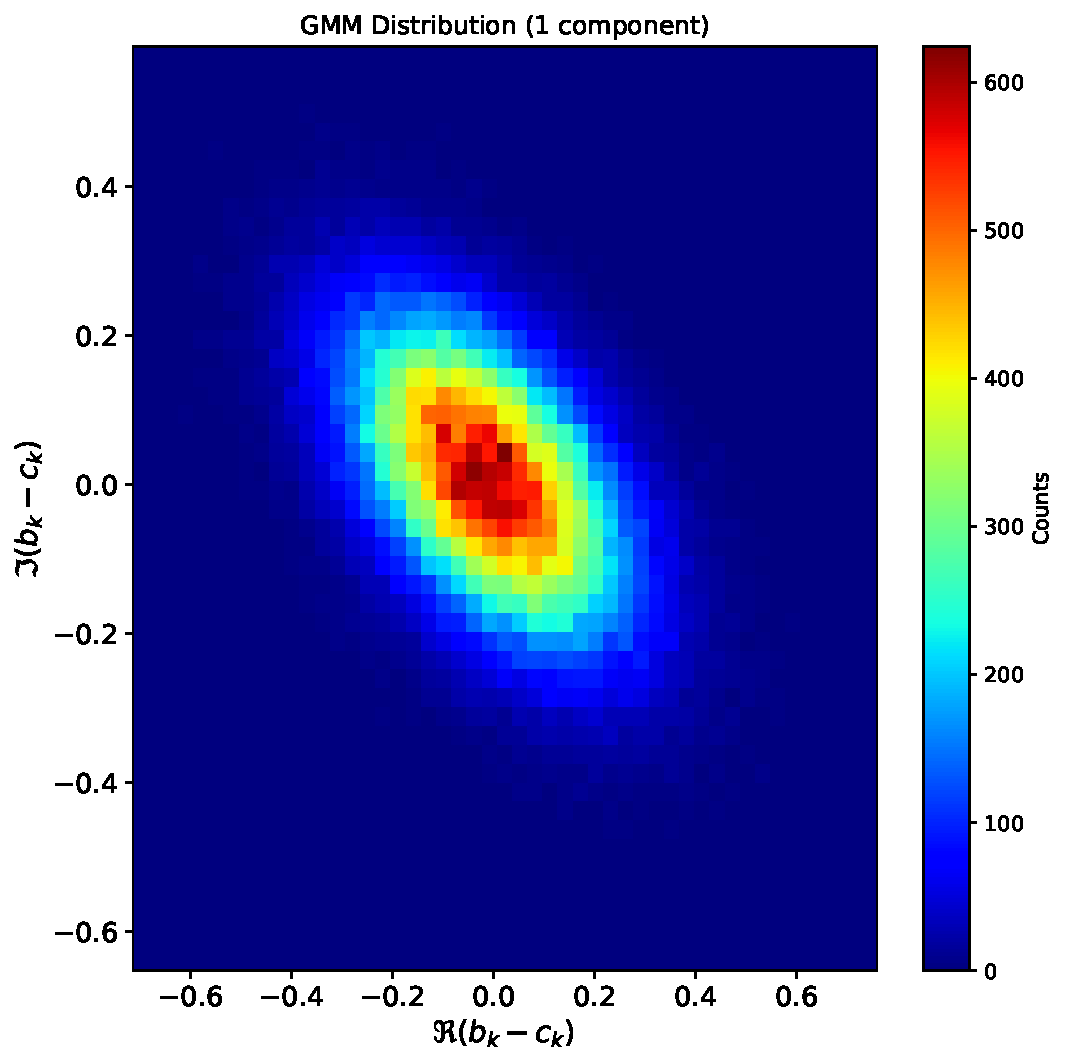
\includegraphics[width=1\linewidth]{images/gauss/gmm_single_fit_triplet_552_dir1_pavedbm-2.pdf} \\
    }
    \end{minipage}
    \begin{minipage}[h]{0.33\linewidth}
    \center{
        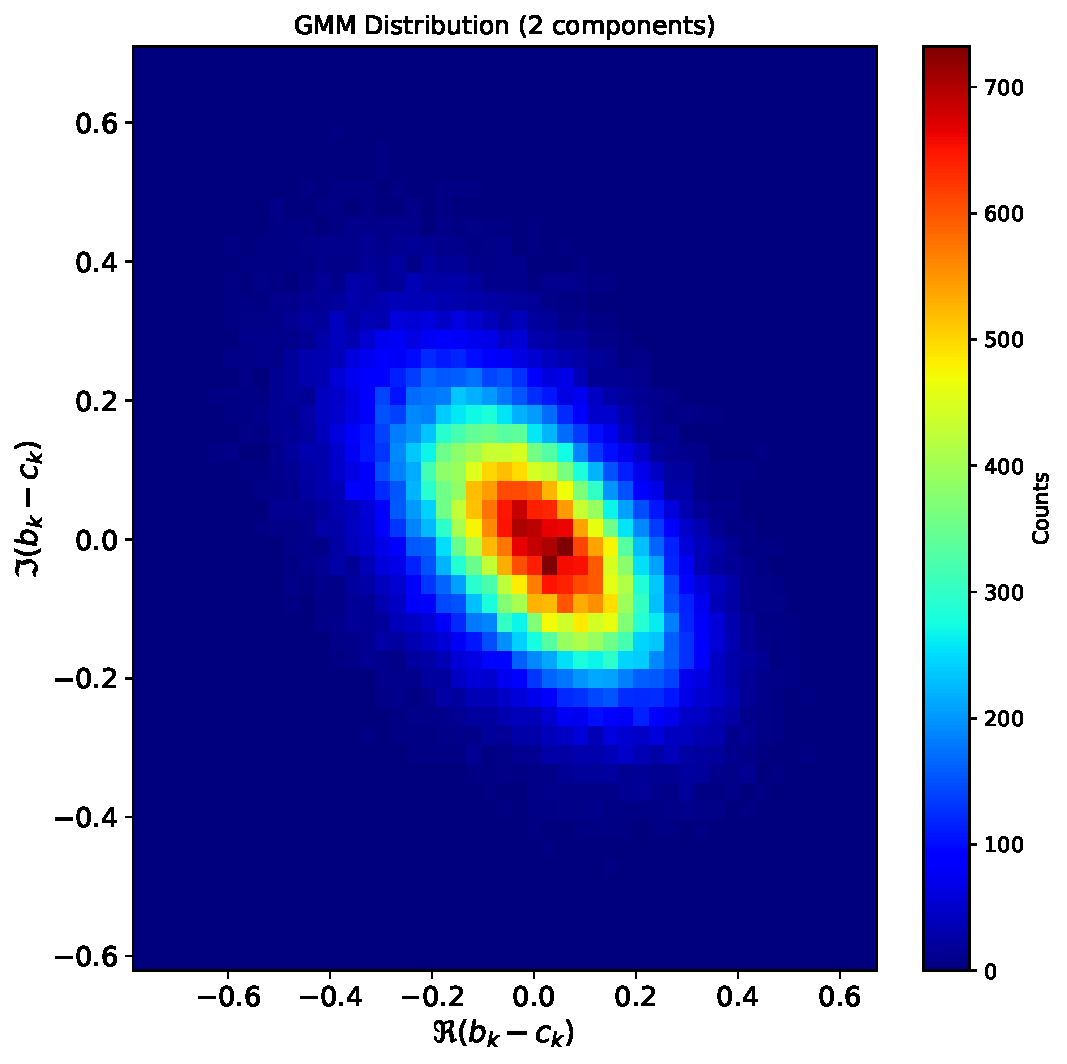
\includegraphics[width=1\linewidth]{images/gauss/gmm_fit_triplet_552_dir1_pavedbm-2.pdf} \\
    }
    \end{minipage}

    \begin{minipage}[h]{0.33\linewidth}
    \center{
        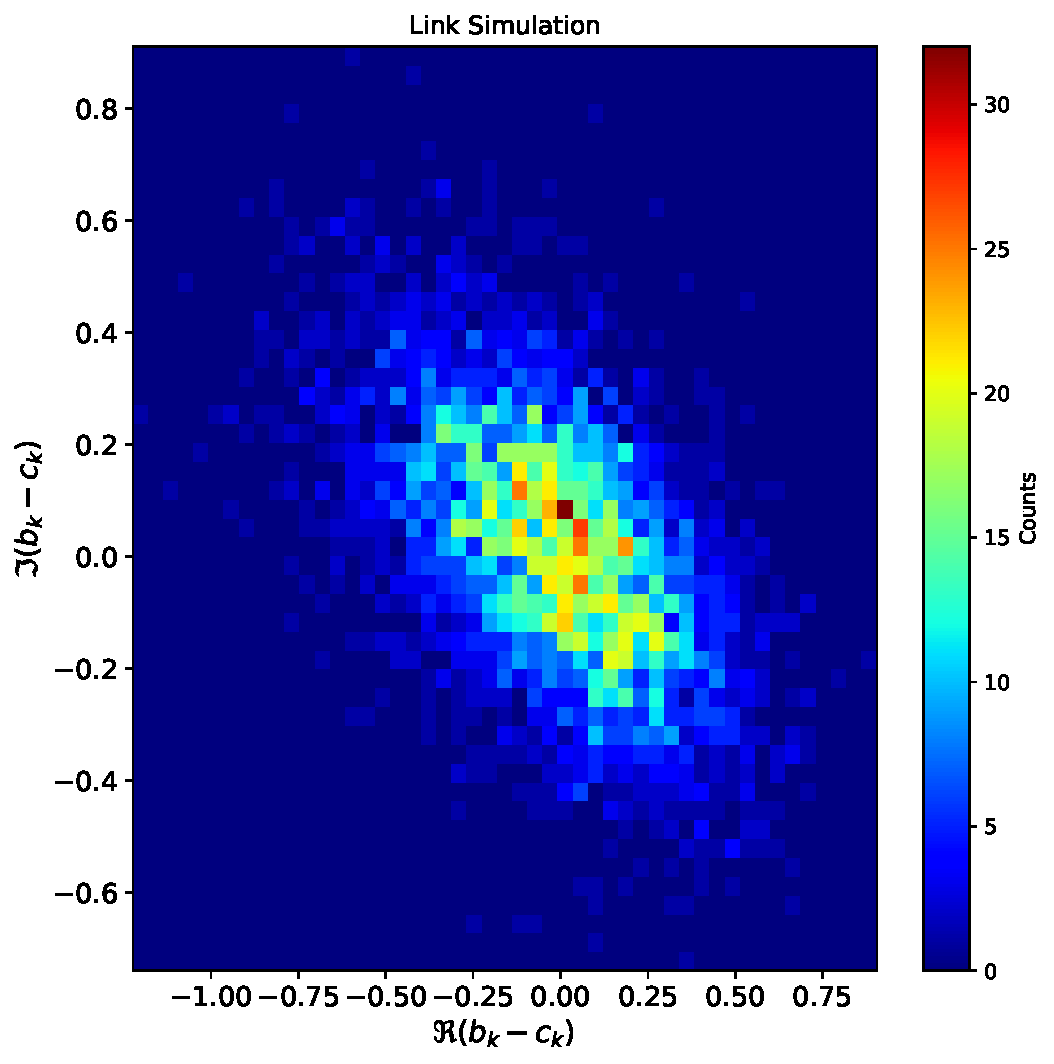
\includegraphics[width=1\linewidth]{images/gauss/exp_fit_triplet_552_dir1_pavedbm0.pdf} \\
    }
    \end{minipage}
    \begin{minipage}[h]{0.33\linewidth}
    \center{
        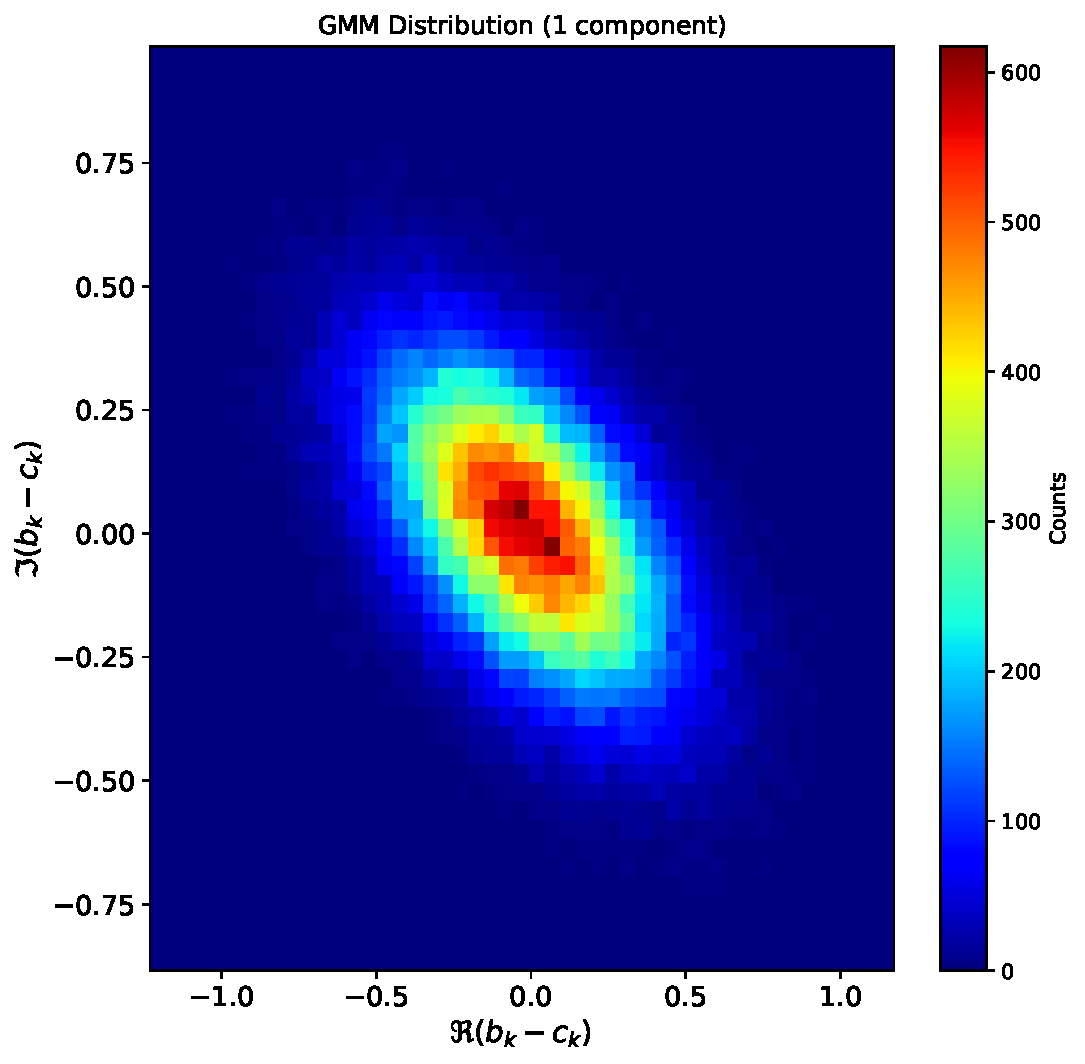
\includegraphics[width=1\linewidth]{images/gauss/gmm_single_fit_triplet_552_dir1_pavedbm0.pdf} \\
    }
    \end{minipage}
    \begin{minipage}[h]{0.33\linewidth}
    \center{
        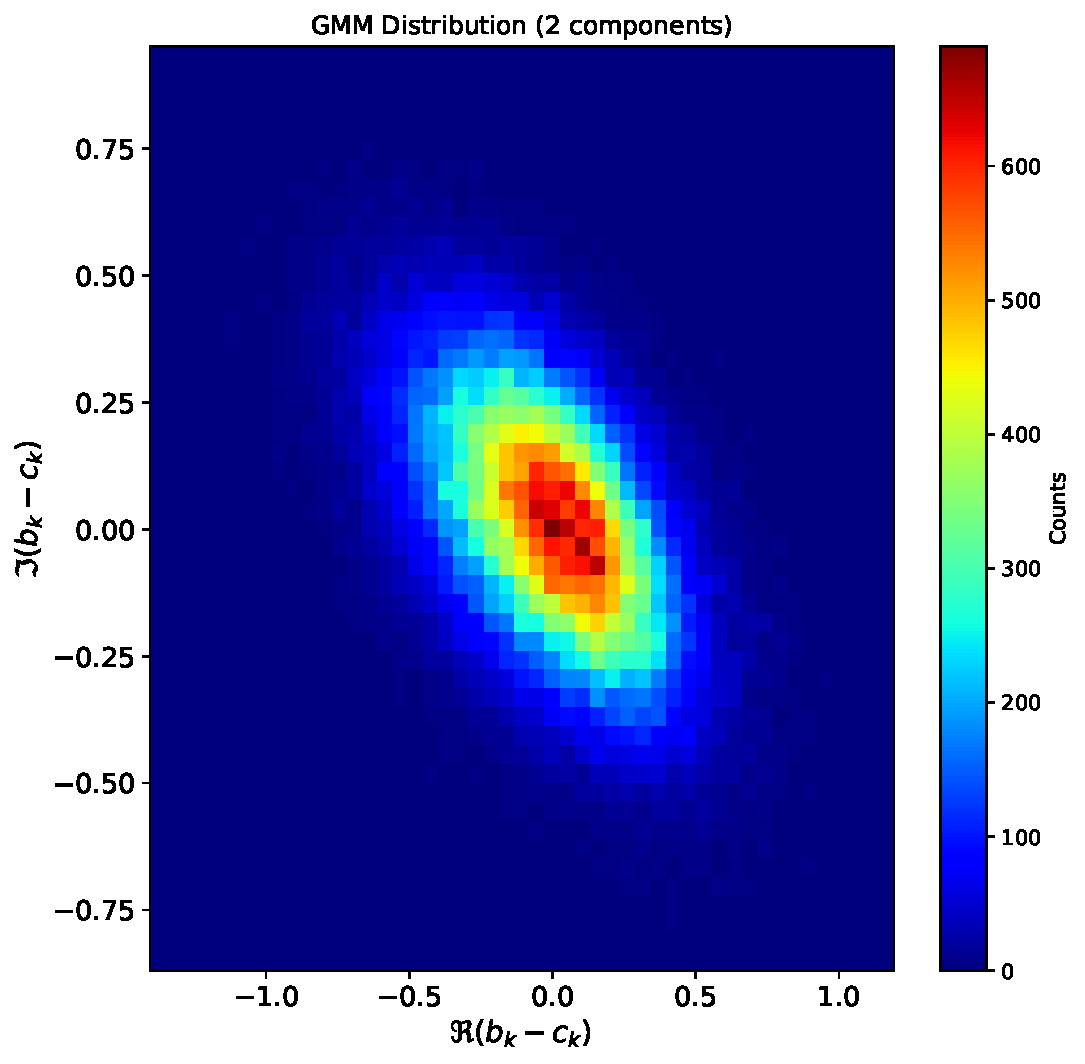
\includegraphics[width=1\linewidth]{images/gauss/gmm_fit_triplet_552_dir1_pavedbm0.pdf} \\
    }
    \end{minipage}

    \begin{minipage}[h]{0.33\linewidth}
    \center{
        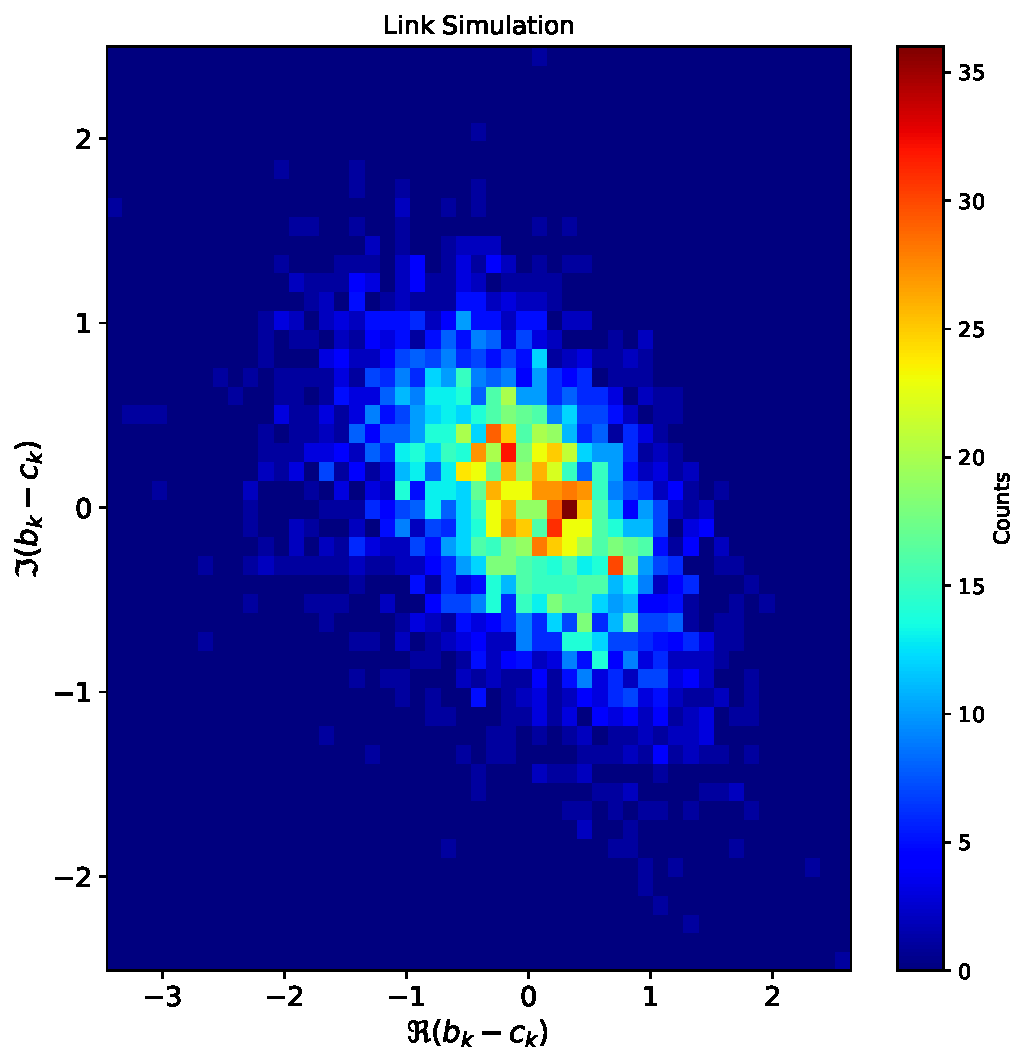
\includegraphics[width=1\linewidth]{images/gauss/exp_fit_triplet_552_dir1_pavedbm4.pdf} \\
    }
    \end{minipage}
    \begin{minipage}[h]{0.33\linewidth}
    \center{
        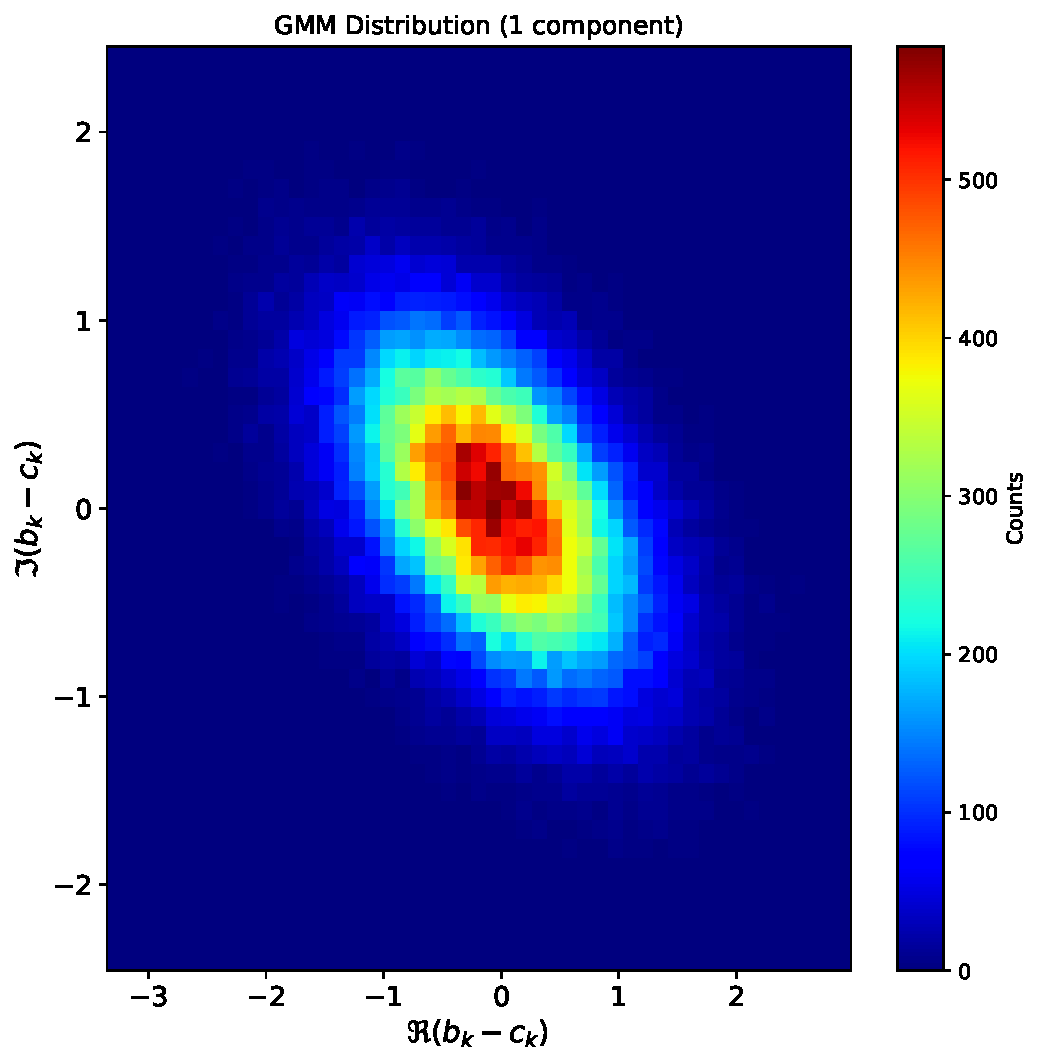
\includegraphics[width=1\linewidth]{images/gauss/gmm_single_fit_triplet_552_dir1_pavedbm4.pdf} \\
    }
    \end{minipage}
    \begin{minipage}[h]{0.33\linewidth}
    \center{
        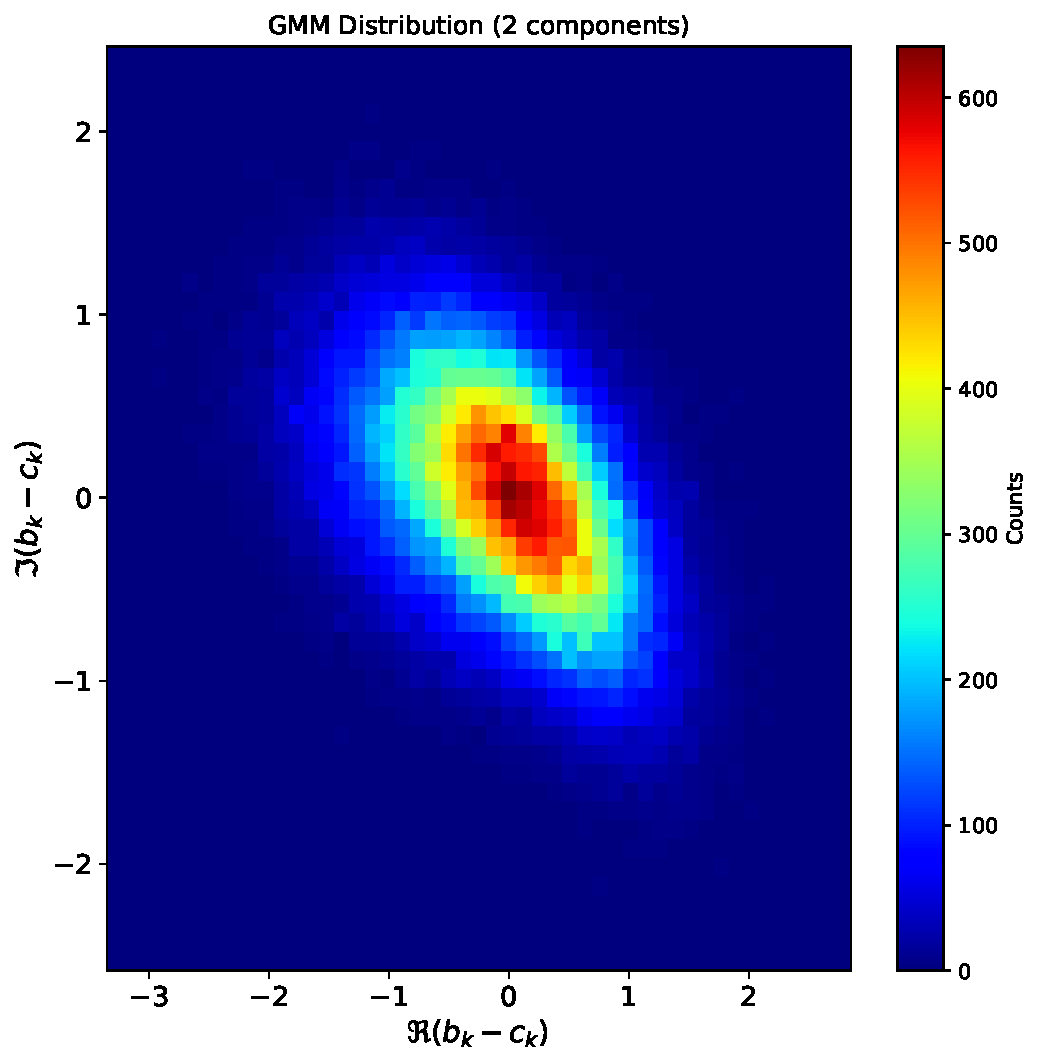
\includegraphics[width=1\linewidth]{images/gauss/gmm_fit_triplet_552_dir1_pavedbm4.pdf} \\
    }
    \end{minipage}

    \begin{minipage}[h]{0.33\linewidth}
    \center{
        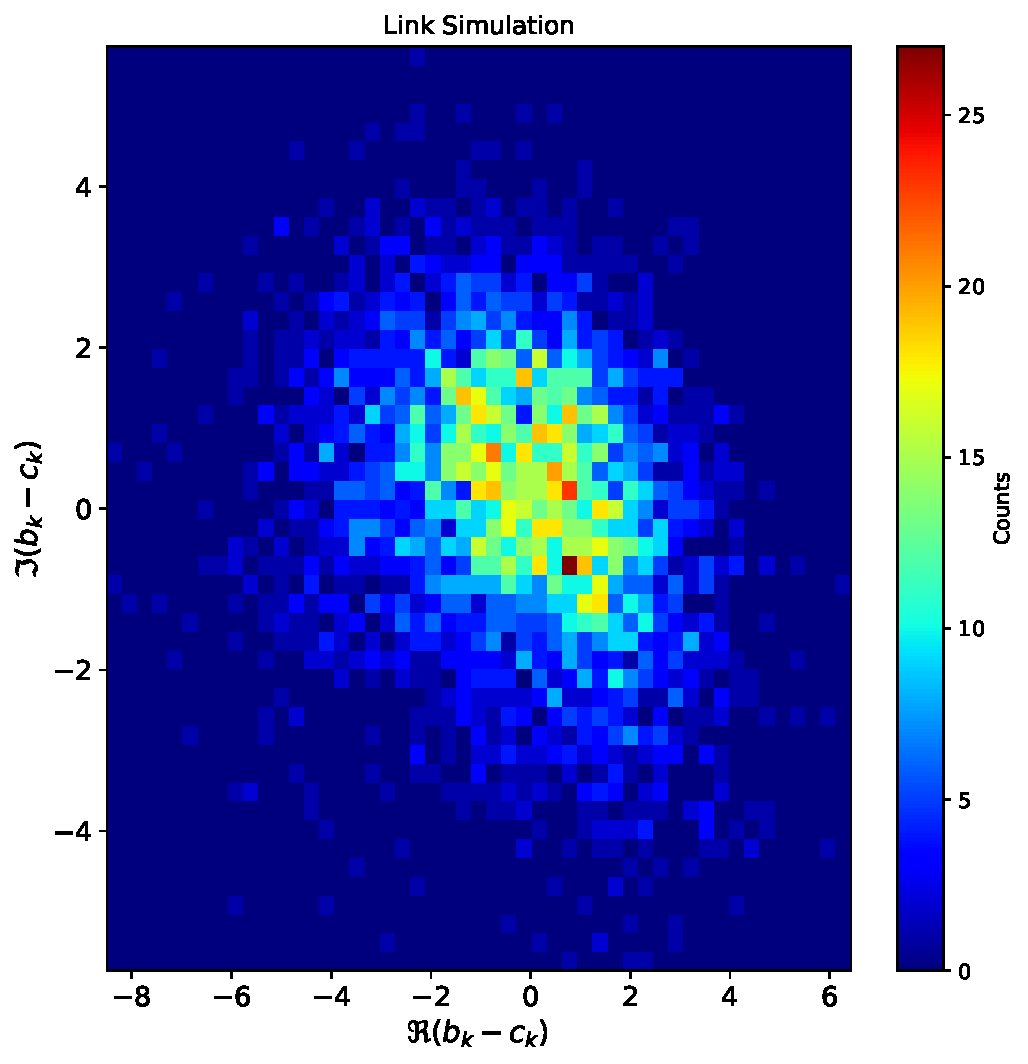
\includegraphics[width=1\linewidth]{images/gauss/exp_fit_triplet_552_dir1_pavedbm8.pdf} \\
    }
    \end{minipage}
    \begin{minipage}[h]{0.33\linewidth}
    \center{
        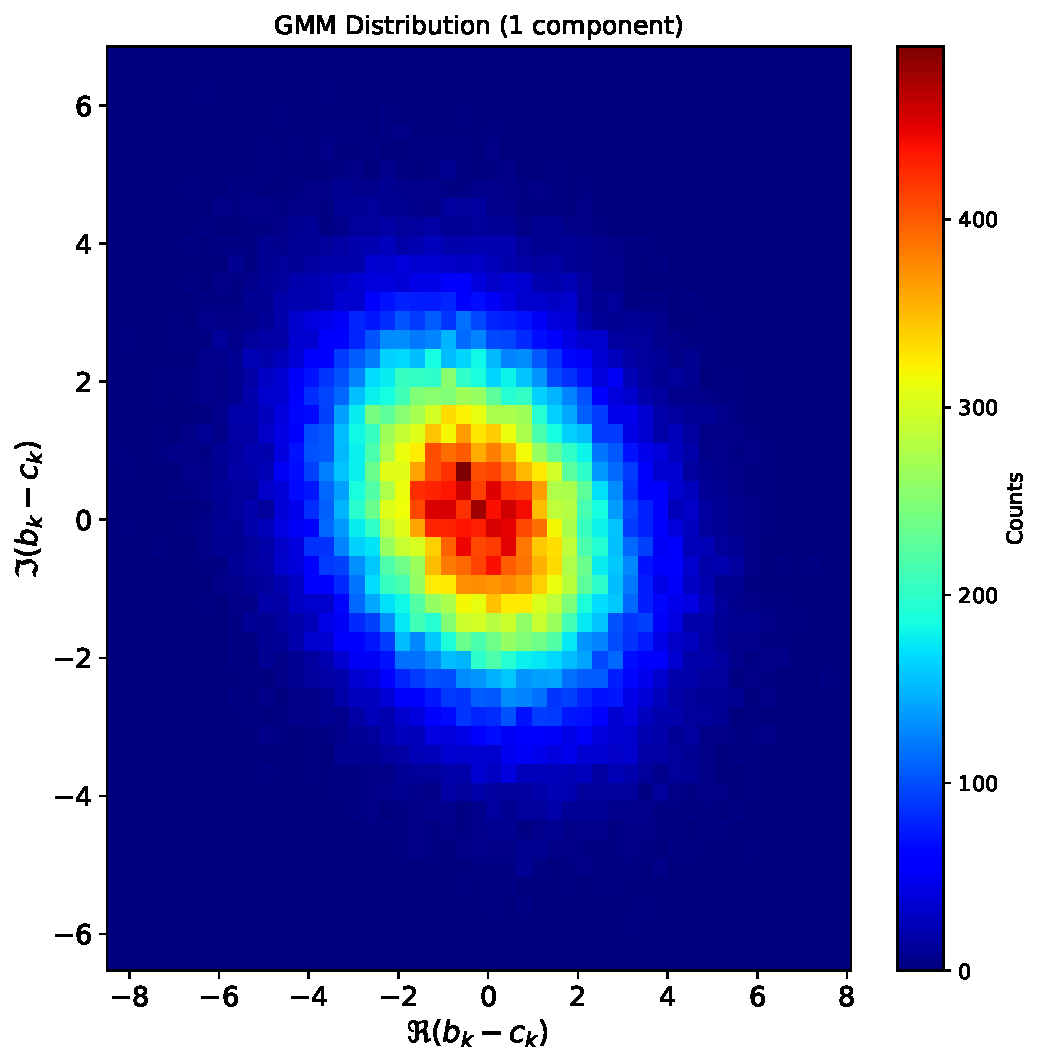
\includegraphics[width=1\linewidth]{images/gauss/gmm_single_fit_triplet_552_dir1_pavedbm8.pdf} \\
    }
    \end{minipage}
    \begin{minipage}[h]{0.33\linewidth}
    \center{
        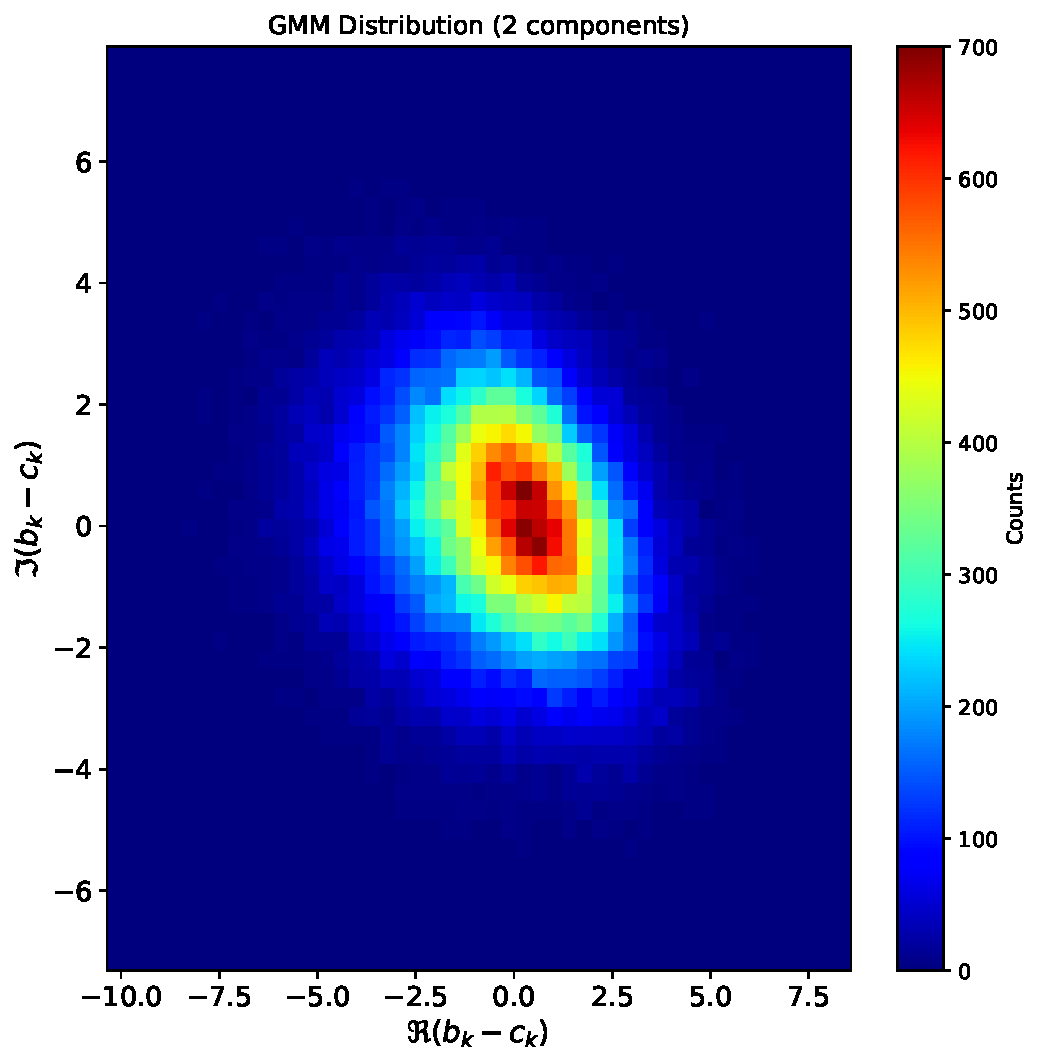
\includegraphics[width=1\linewidth]{images/gauss/gmm_fit_triplet_552_dir1_pavedbm8.pdf} \\
    }
    \end{minipage}
    \caption{The distributions of the received constellation points \( b_k \), centered with respect to the transmitted symbol \( c_k \) for triplet 552 $[1+3\mathrm{i}, 1+3\mathrm{i}, 3+1\mathrm{i}]$. The first column illustrates the distribution of simulation data for a real communication system. The second column represents the distribution fitted with a single two-dimensional Gaussian distribution, while the third column visualizes a mixture of two Gaussians.}
    \label{fig:gauss_triplet_552_compare_2d}
\end{figure}

\begin{figure}[hp]
    \begin{minipage}[h]{0.33\linewidth}
    \center{
        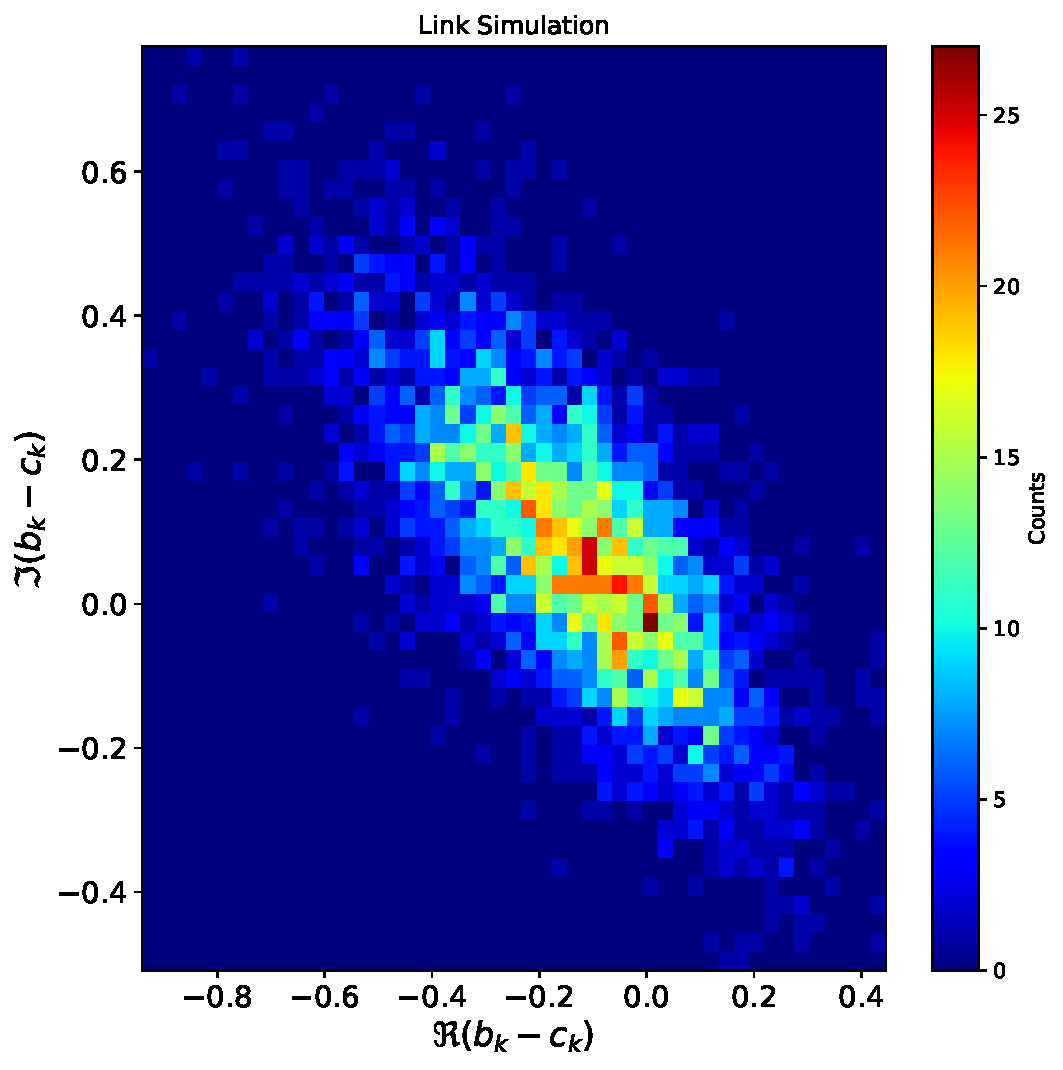
\includegraphics[width=1\linewidth]{images/gauss/bigf_exp_fit_triplet_2730_dir1_pavedbm-2.pdf} \\
    }
    \end{minipage}
    \begin{minipage}[h]{0.33\linewidth}
    \center{
        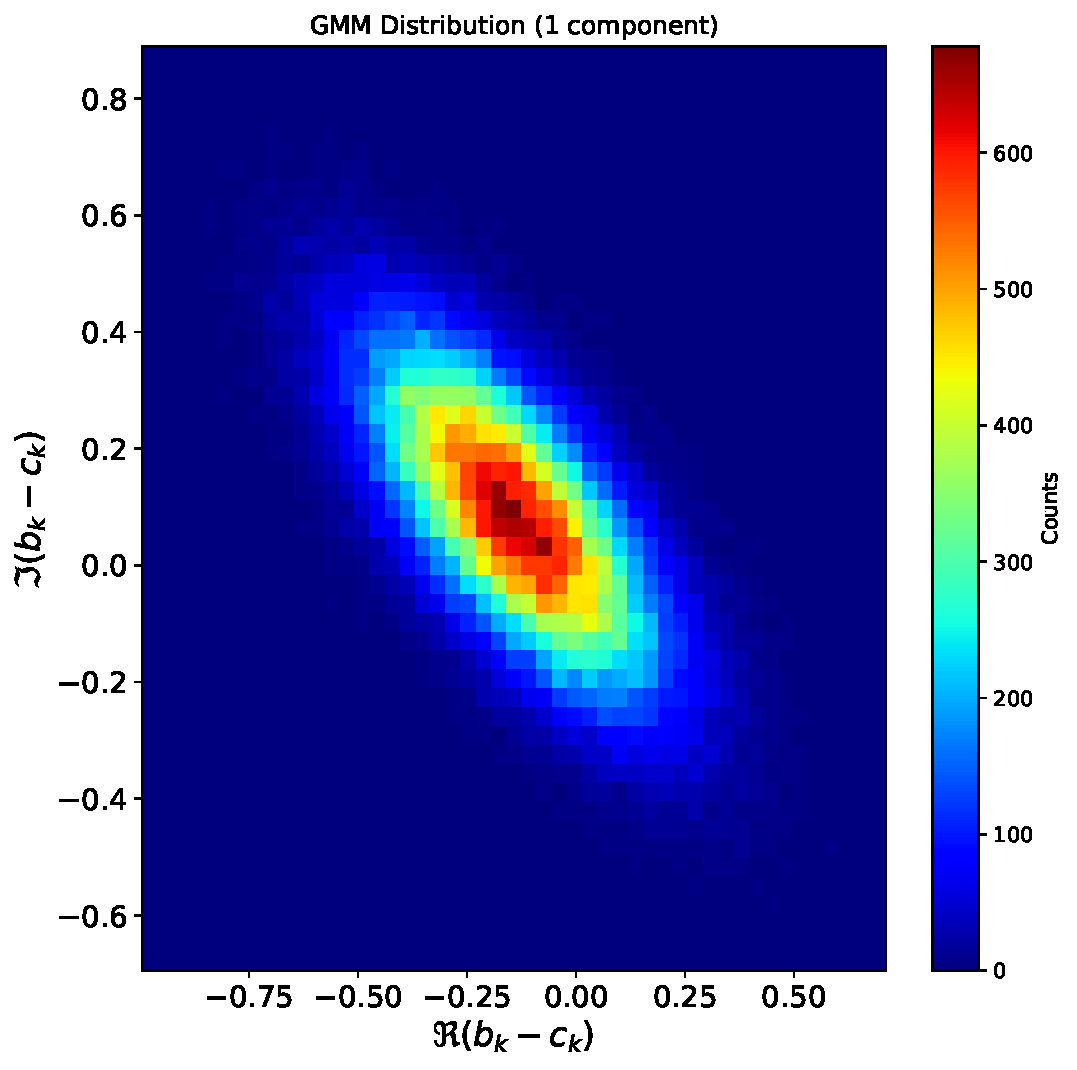
\includegraphics[width=1\linewidth]{images/gauss/bigf_gmm_single_fit_triplet_2730_dir1_pavedbm-2.pdf} \\
    }
    \end{minipage}
    \begin{minipage}[h]{0.33\linewidth}
    \center{
        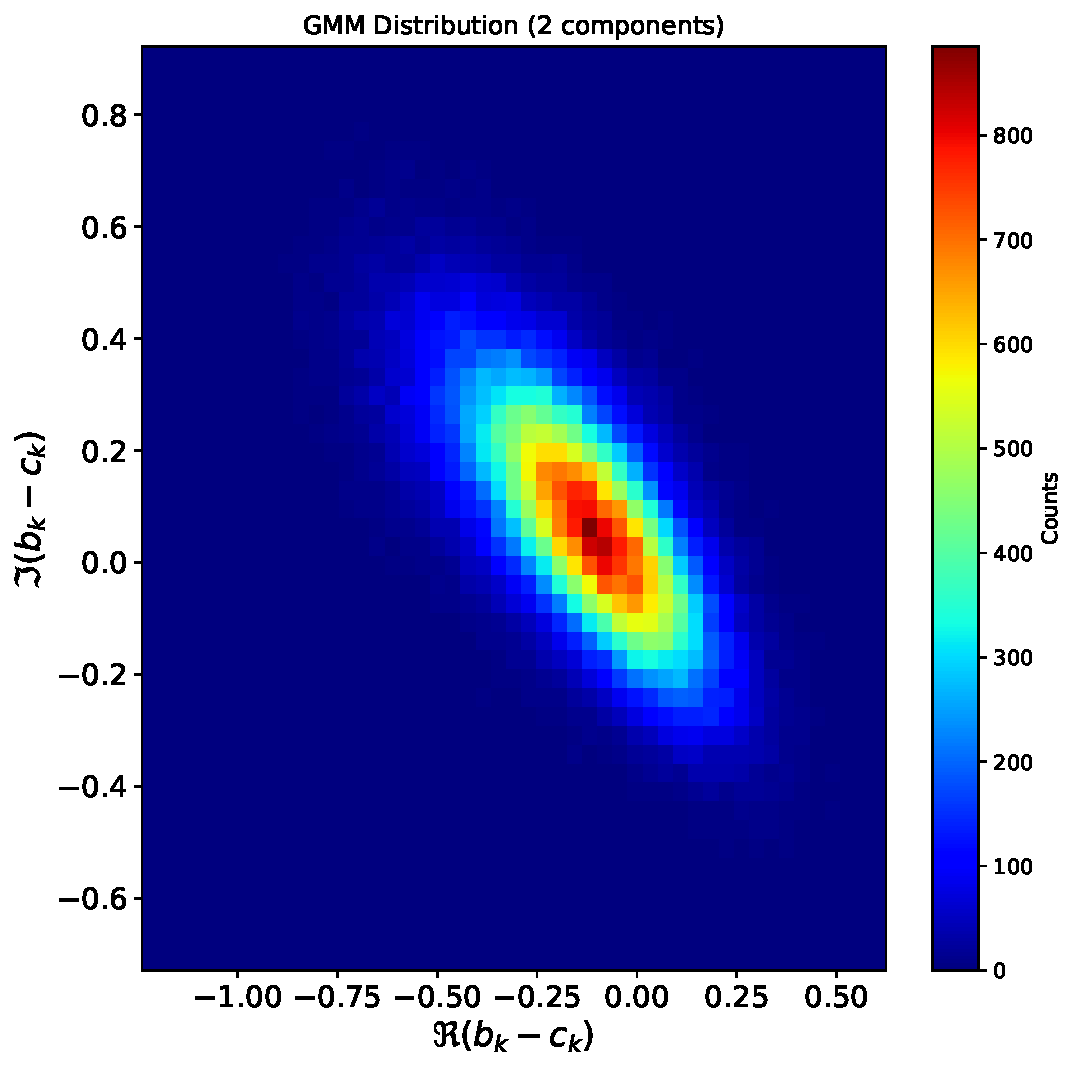
\includegraphics[width=1\linewidth]{images/gauss/bigf_gmm_fit_triplet_2730_dir1_pavedbm-2.pdf} \\
    }
    \end{minipage}

    \begin{minipage}[h]{0.33\linewidth}
    \center{
        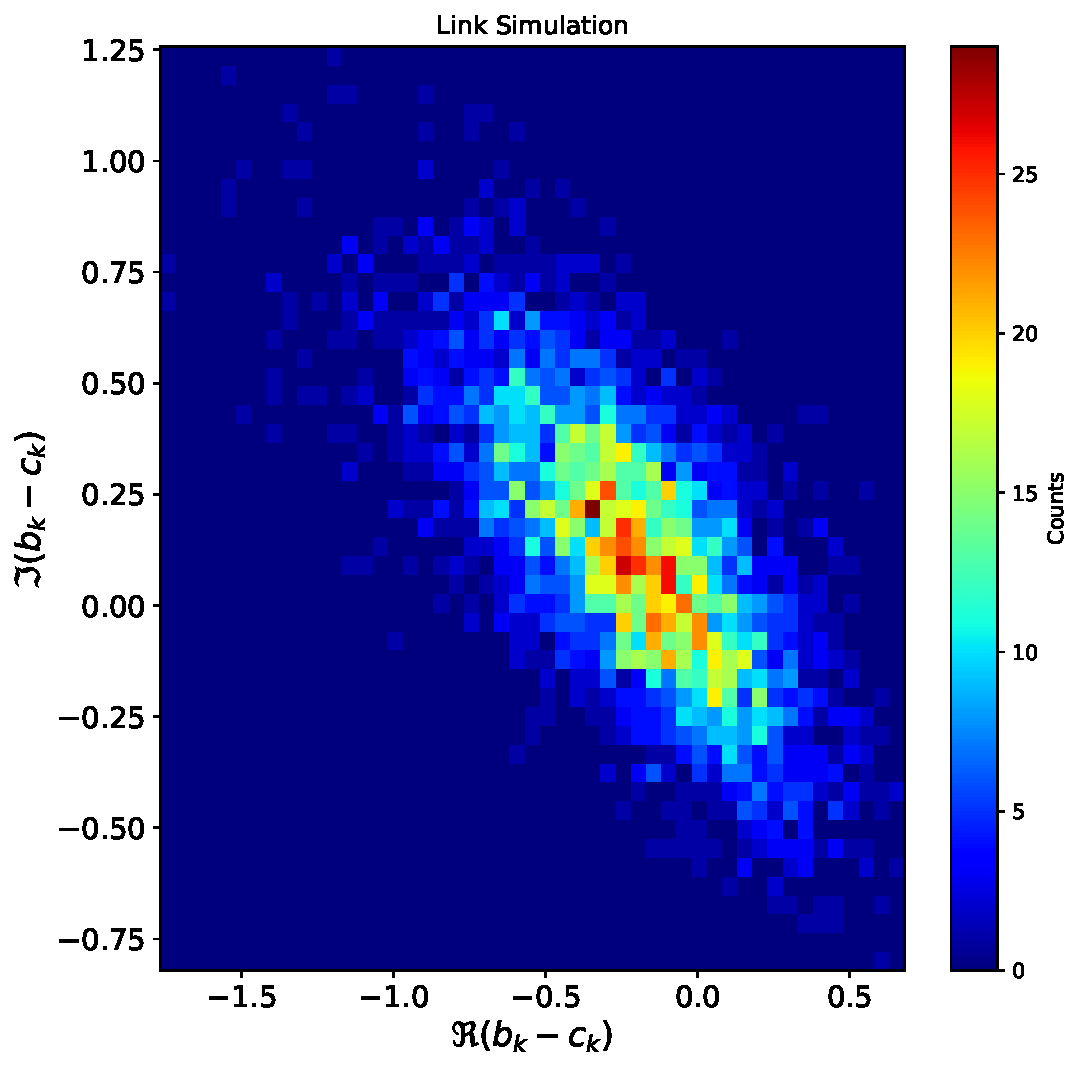
\includegraphics[width=1\linewidth]{images/gauss/bigf_exp_fit_triplet_2730_dir1_pavedbm0.pdf} \\
    }
    \end{minipage}
    \begin{minipage}[h]{0.33\linewidth}
    \center{
        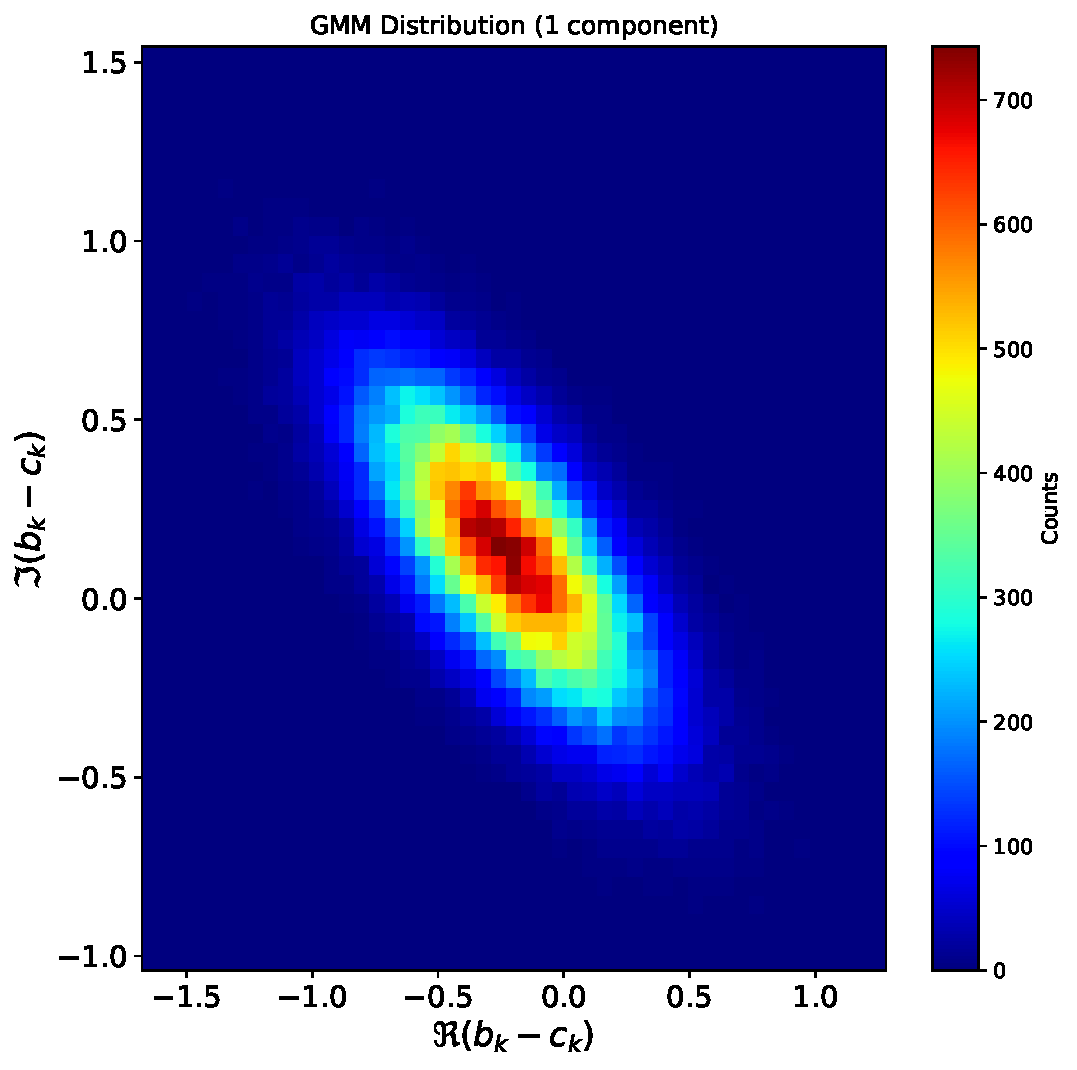
\includegraphics[width=1\linewidth]{images/gauss/bigf_gmm_single_fit_triplet_2730_dir1_pavedbm0.pdf} \\
    }
    \end{minipage}
    \begin{minipage}[h]{0.33\linewidth}
    \center{
        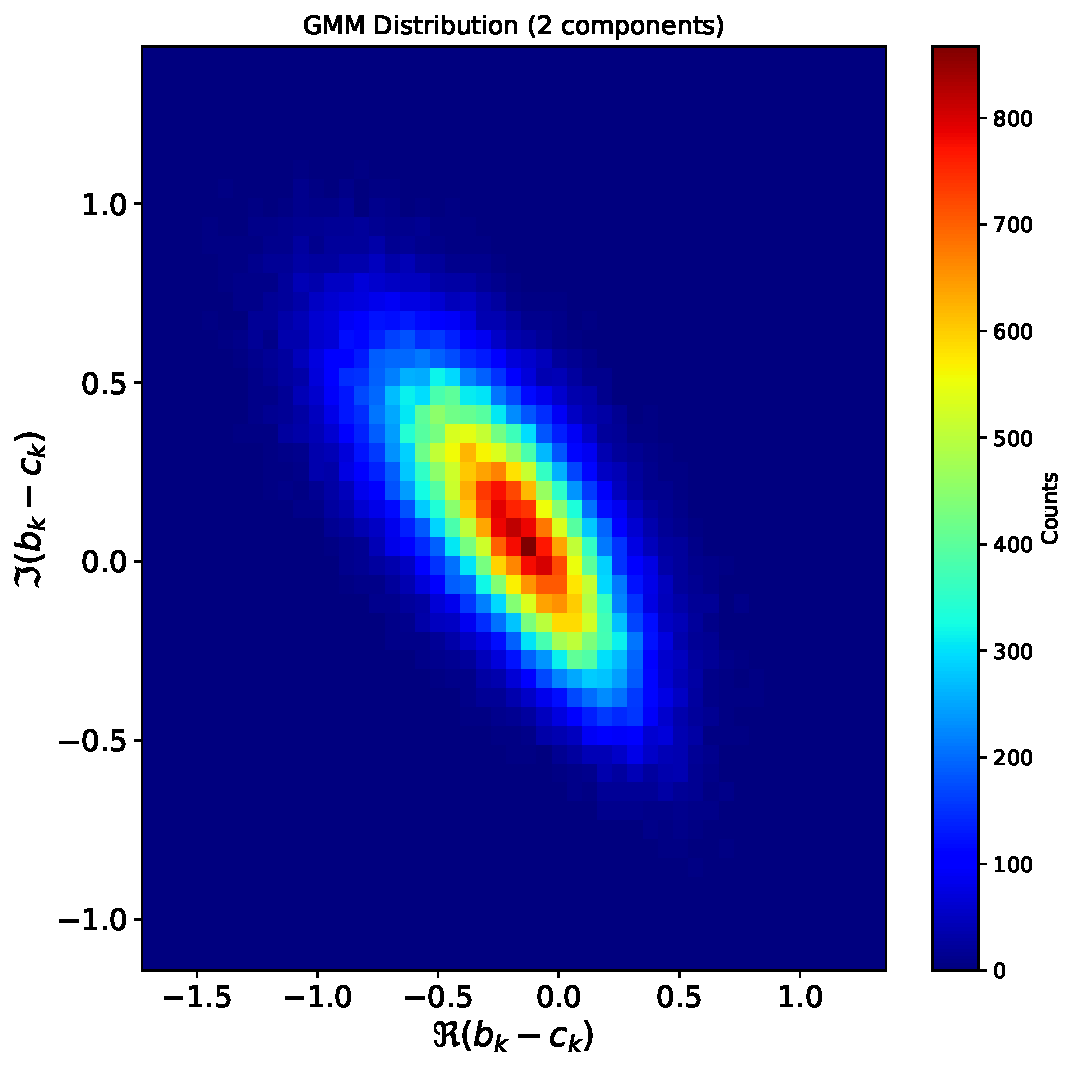
\includegraphics[width=1\linewidth]{images/gauss/bigf_gmm_fit_triplet_2730_dir1_pavedbm0.pdf} \\
    }
    \end{minipage}

    \begin{minipage}[h]{0.33\linewidth}
    \center{
        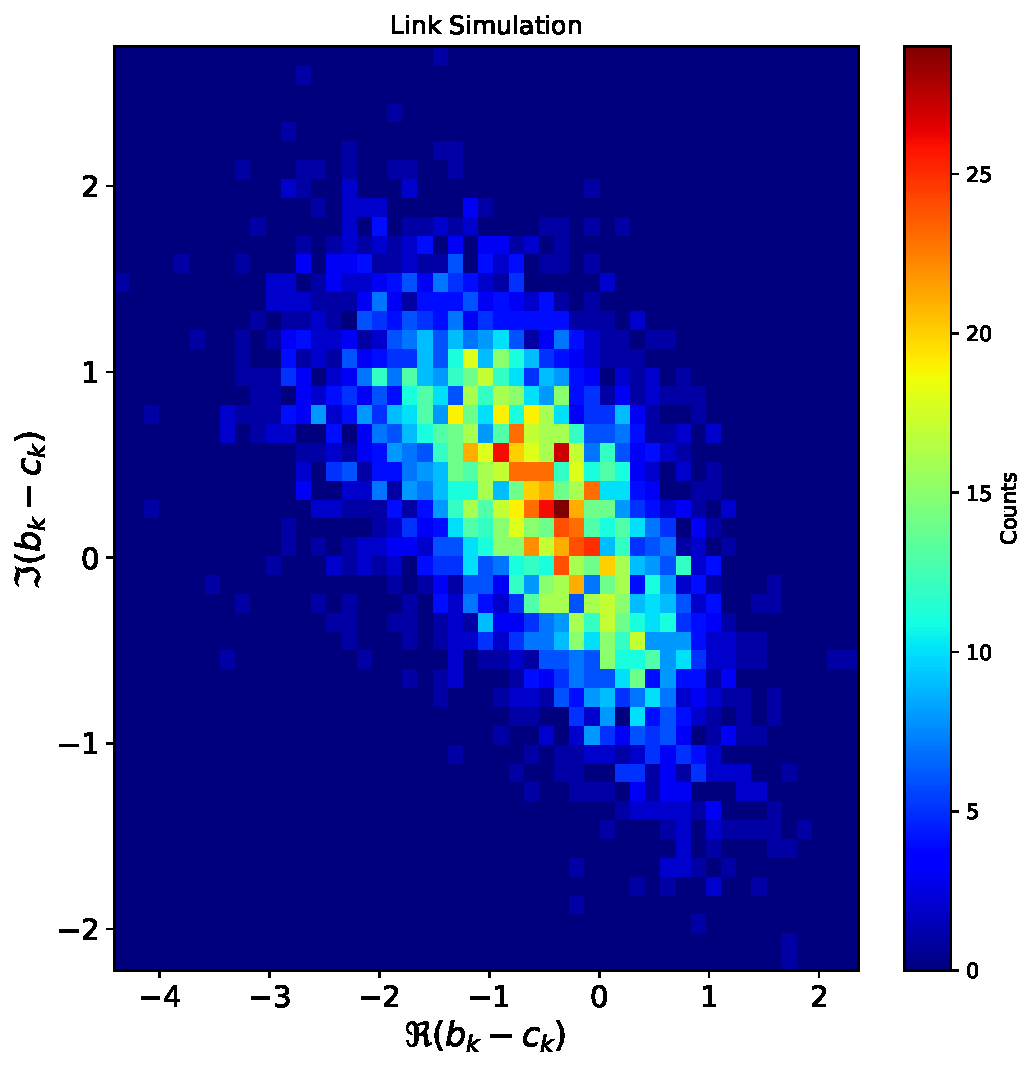
\includegraphics[width=1\linewidth]{images/gauss/bigf_exp_fit_triplet_2730_dir1_pavedbm4.pdf} \\
    }
    \end{minipage}
    \begin{minipage}[h]{0.33\linewidth}
    \center{
        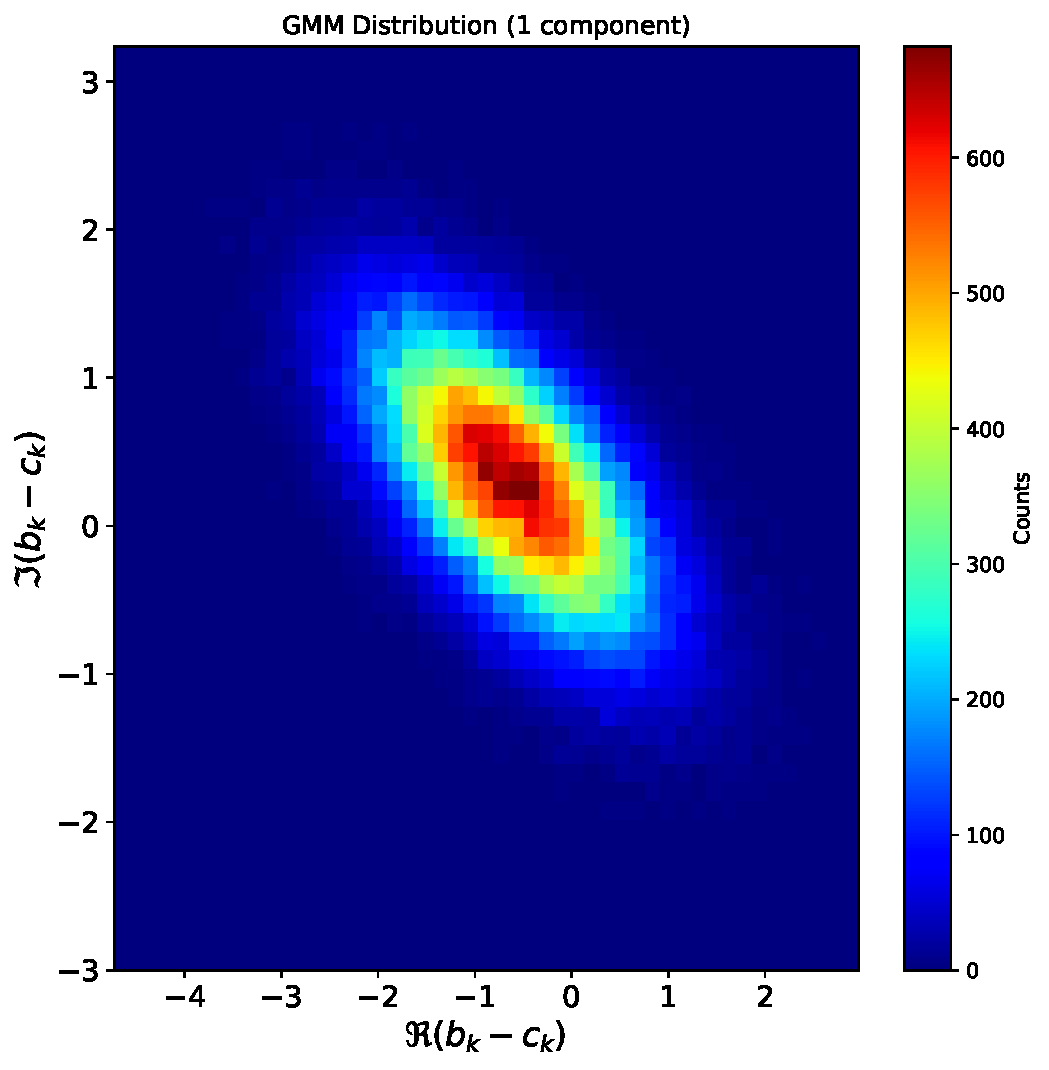
\includegraphics[width=1\linewidth]{images/gauss/bigf_gmm_single_fit_triplet_2730_dir1_pavedbm4.pdf} \\
    }
    \end{minipage}
    \begin{minipage}[h]{0.33\linewidth}
    \center{
        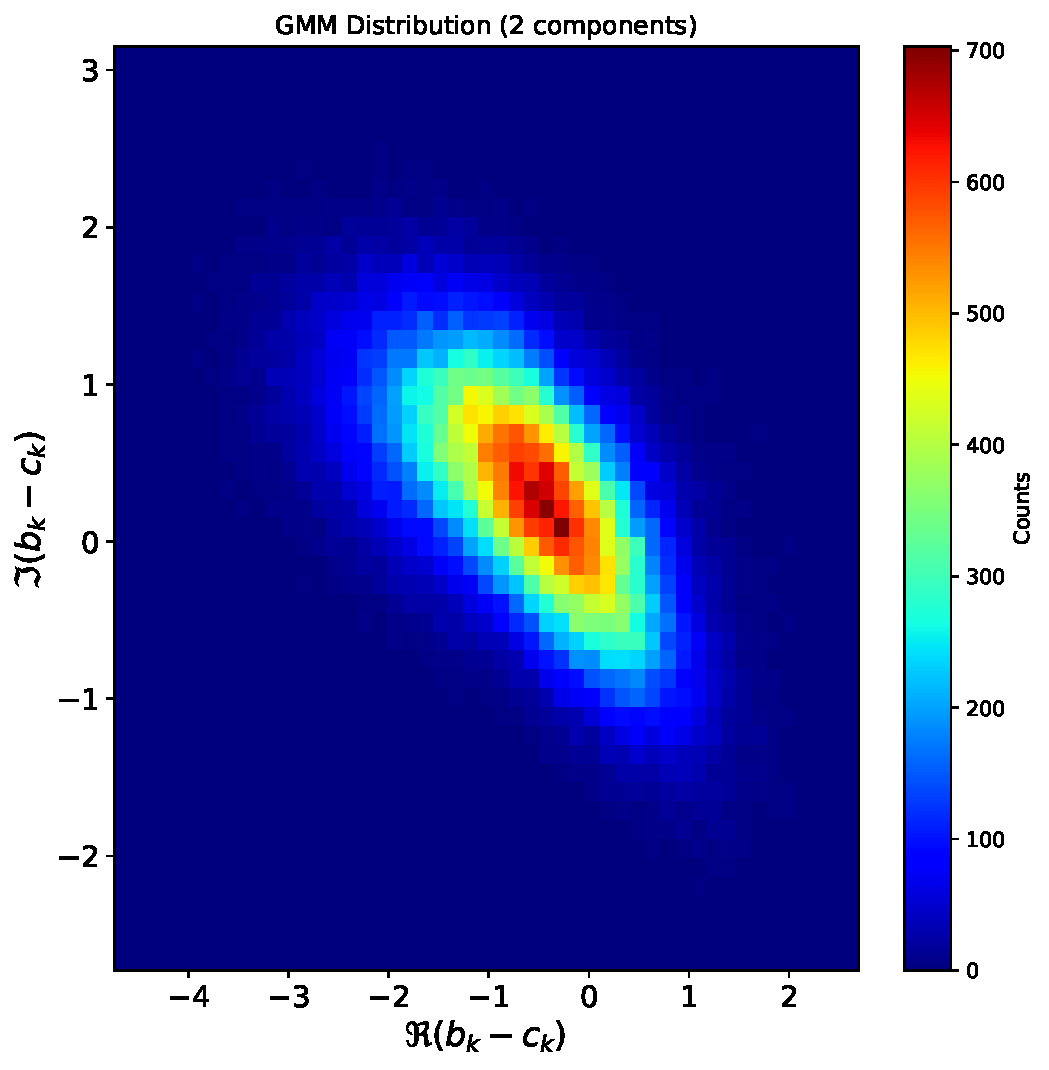
\includegraphics[width=1\linewidth]{images/gauss/bigf_gmm_fit_triplet_2730_dir1_pavedbm4.pdf} \\
    }
    \end{minipage}

    \begin{minipage}[h]{0.33\linewidth}
    \center{
        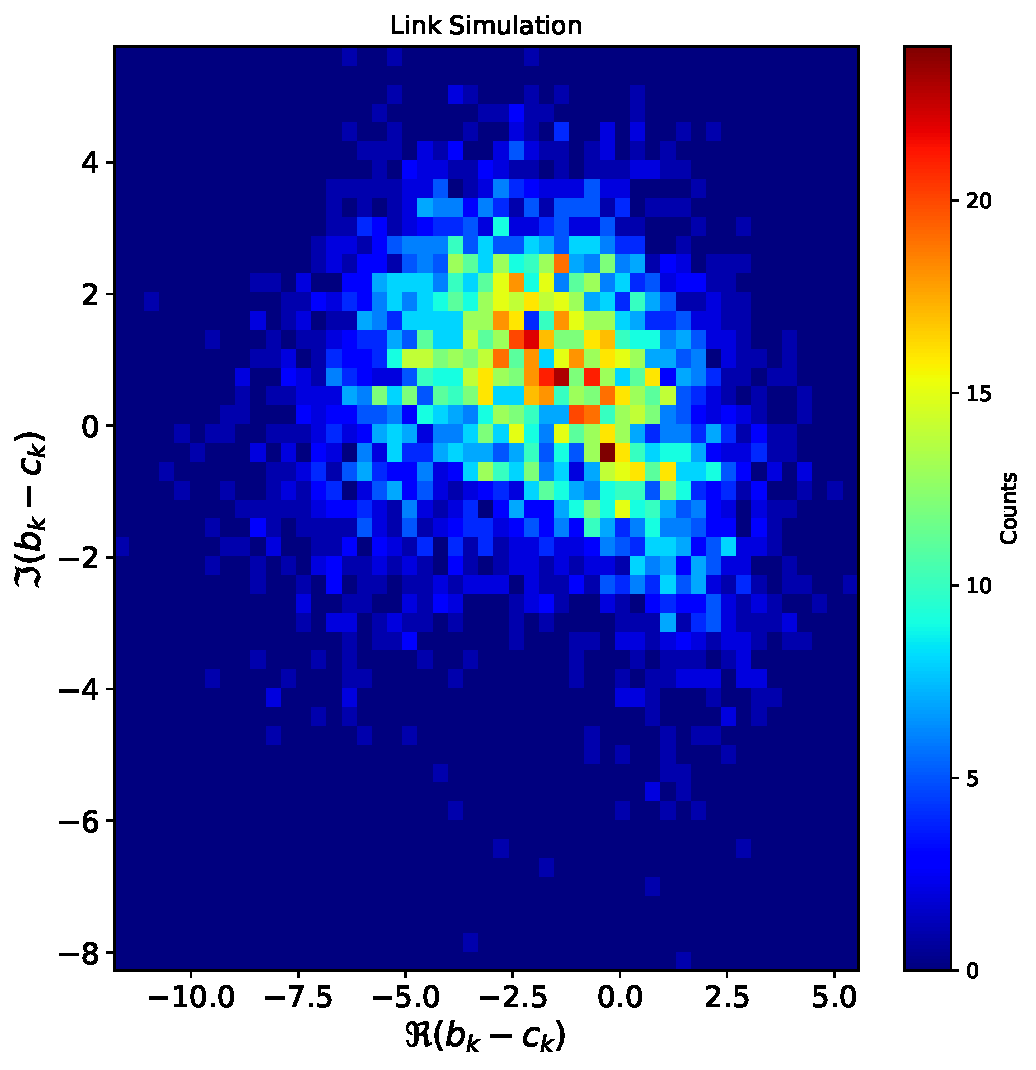
\includegraphics[width=1\linewidth]{images/gauss/bigf_exp_fit_triplet_2730_dir1_pavedbm8.pdf} \\
    }
    \end{minipage}
    \begin{minipage}[h]{0.33\linewidth}
    \center{
        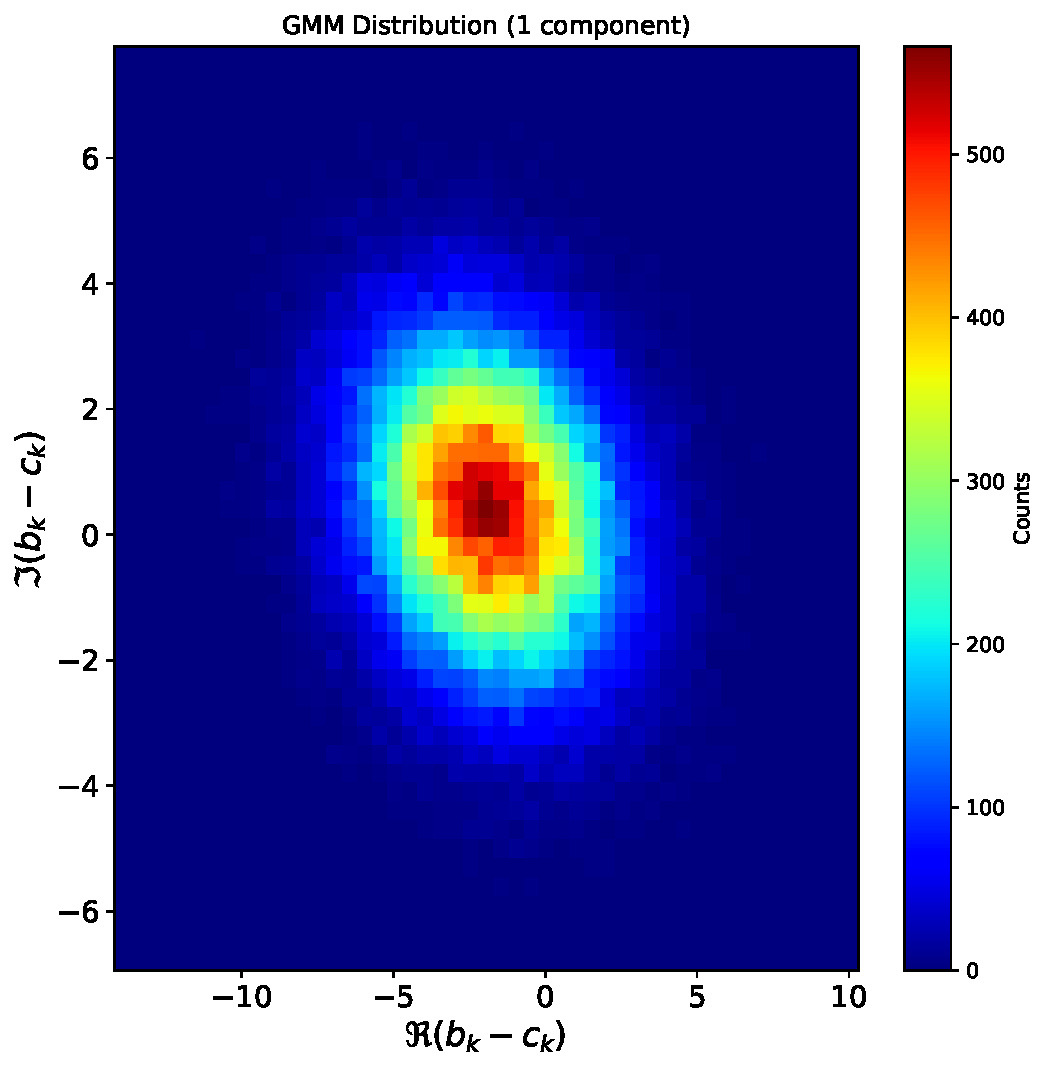
\includegraphics[width=1\linewidth]{images/gauss/bigf_gmm_single_fit_triplet_2730_dir1_pavedbm8.pdf} \\
    }
    \end{minipage}
    \begin{minipage}[h]{0.33\linewidth}
    \center{
        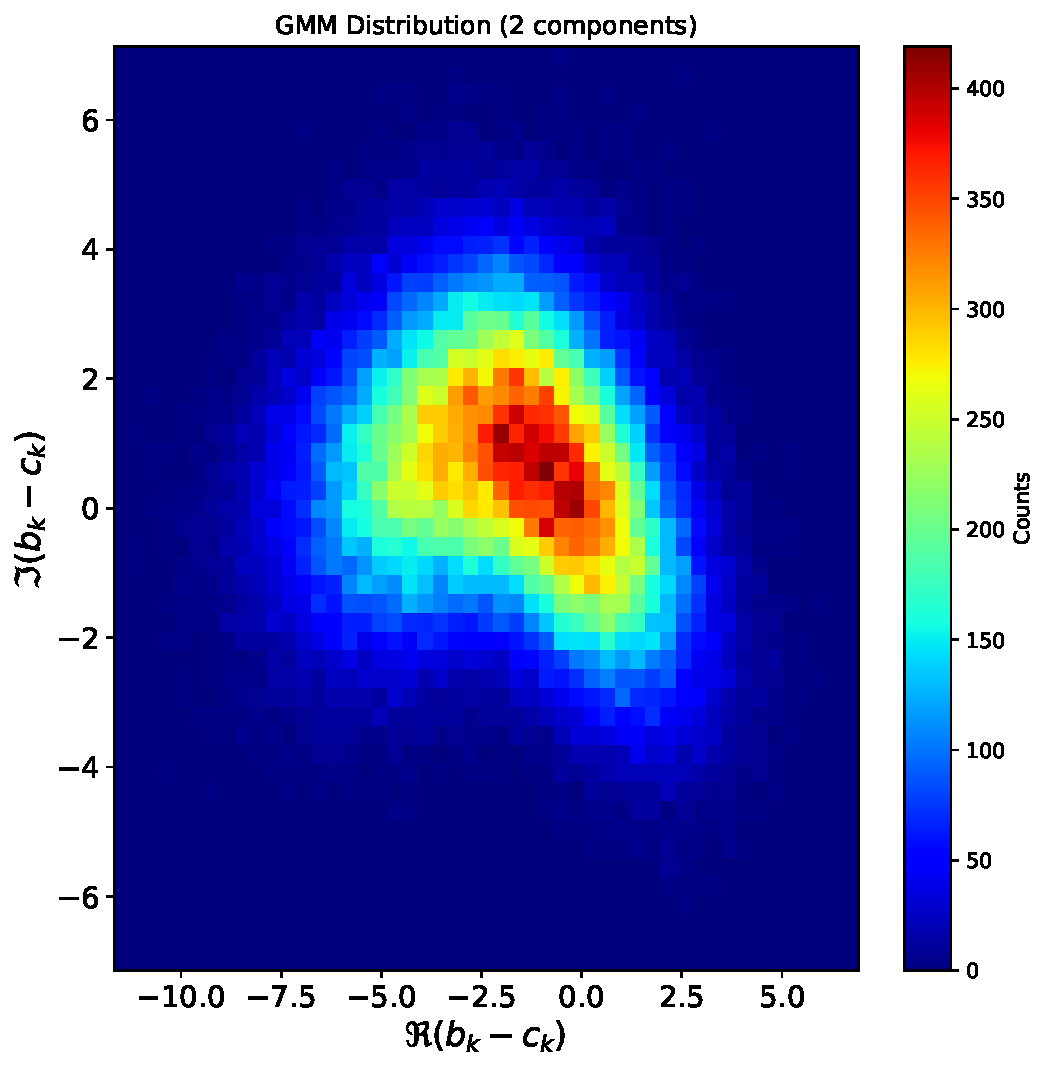
\includegraphics[width=1\linewidth]{images/gauss/bigf_gmm_fit_triplet_2730_dir1_pavedbm8.pdf} \\
    }
    \end{minipage}
    \caption{The distributions of the received constellation points \( b_k \), centered with respect to the transmitted symbol \( c_k \) for triplet 2730 $[3+3\mathrm{i}, 3+3\mathrm{i}, 3+3\mathrm{i}]$. The first column illustrates the distribution of simulation data for a real communication system. The second column represents the distribution fitted with a single two-dimensional Gaussian distribution, while the third column visualizes a mixture of two Gaussians.}
    \label{fig:gauss_triplet_2730_compare_2d}
\end{figure}

After the comprehensive data collection and fitting of distributions for all conceivable triplets, we begin our discussion with visual illustrations.

Figures~\ref{fig:gauss_triplet_552_compare_2d} and~\ref{fig:gauss_triplet_2730_compare_2d} depict the distributions of the received constellation points \( b_k \), centered with respect to the transmitted symbol \( c_k \) (after \gls{cdc} and \gls{npe}). Essentially, these figures represent the received symbols after subtracting the original transmitted symbol, corresponding to specific ``triplets''. Figure~\ref{fig:gauss_triplet_552_compare_2d} presents the distribution for triplet 552, whereas Figure~\ref{fig:gauss_triplet_2730_compare_2d} displays the distribution for triplet 2730. Notably, these distributions arise from nonlinear effects during the propagation of the \acrshort{wdm} signal through the optical fiber, as the system excludes additional noise from \acrshort{edfa} amplifiers.

Both Figures~\ref{fig:gauss_triplet_552_compare_2d} and~\ref{fig:gauss_triplet_2730_compare_2d} are structured as follows: rows correspond to different average signal power levels (first row at \(-2\) dBm, second at \(0\) dBm, third at \(4\) dBm, and fourth at \(8\) dBm). The first column illustrates the distribution of simulation data for a real communication system with the aforementioned parameters. These distributions are then fitted with a \gls{gmm}, and the derived parameters are used to generate the visualizations in the second and third columns. The second column represents the distribution fitted with a single two-dimensional Gaussian distribution, while the third column visualizes a mixture of two Gaussians, each column containing \(100000\) randomly generated points.

Examining Figure~\ref{fig:gauss_triplet_552_compare_2d}, at low average signal power, the \acrshort{gmm}s with one and two components appear similar; however, the distribution for a single-component \acrshort{gmm} is broader, indicating discernible differences. At \(0\) dBm average power, the distinction remains, though both distributions seem to fit the simulation reasonably well. The disparity becomes more visible at higher power levels, where the two-component \acrshort{gmm} notably deviates from a Gaussian shape.

A comparable behaviour we can see for triplet 2730 in Figure~\ref{fig:gauss_triplet_2730_compare_2d}. At lower average signal powers, the distributions vary but are distinct. A striking example is at the highest power level (last row), where both the simulation distribution and the \acrshort{gmm} with two components form a distinctive shape of a German pretzel. It is evident that a single-component \acrshort{gmm} fails to accurately represent this distribution.

These figures are merely exemplars out of \(4096\) different triplet distributions, yet they offer a compelling demonstration that the internal structure of distributions can be intricate and extend well beyond simple Gaussian forms.


\begin{figure}[tp]
    \begin{minipage}[h]{0.5\linewidth}
    \center{
        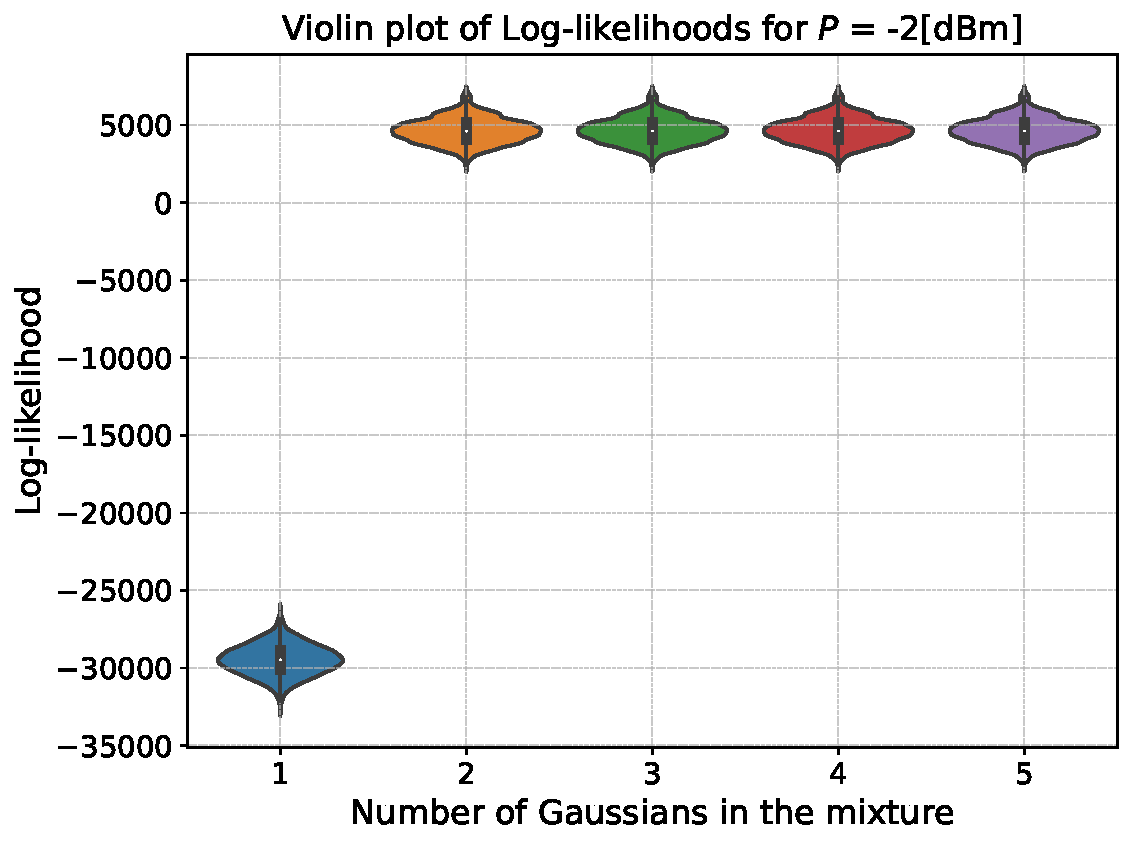
\includegraphics[width=1\linewidth]{images/gauss/bigf_loglik_pdbm_-2.pdf} (a) \\
    }
    \end{minipage}
    \begin{minipage}[h]{0.5\linewidth}
    \center{
        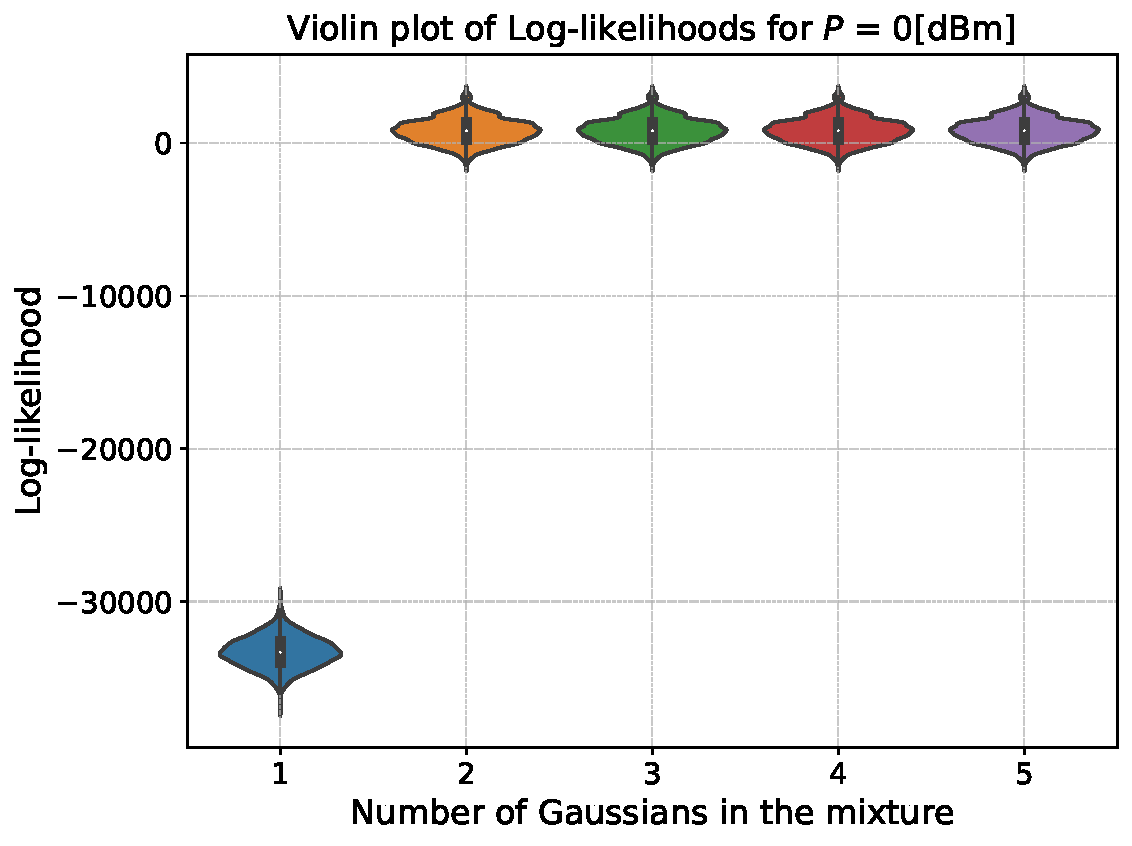
\includegraphics[width=1\linewidth]{images/gauss/bigf_loglik_pdbm_0.pdf} (b) \\
    }
    \end{minipage}

    \begin{minipage}[h]{0.5\linewidth}
    \center{
        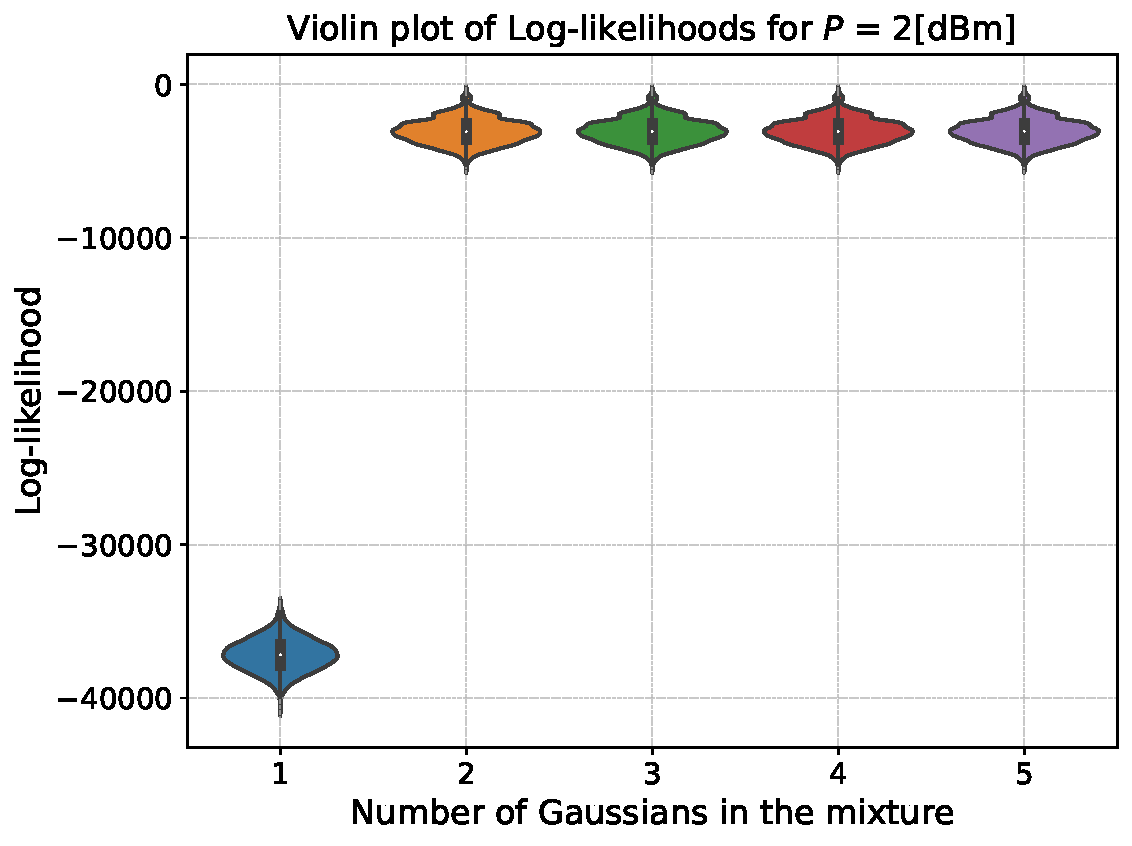
\includegraphics[width=1\linewidth]{images/gauss/bigf_loglik_pdbm_2.pdf} (c) \\
    }
    \end{minipage}
    \begin{minipage}[h]{0.5\linewidth}
    \center{
        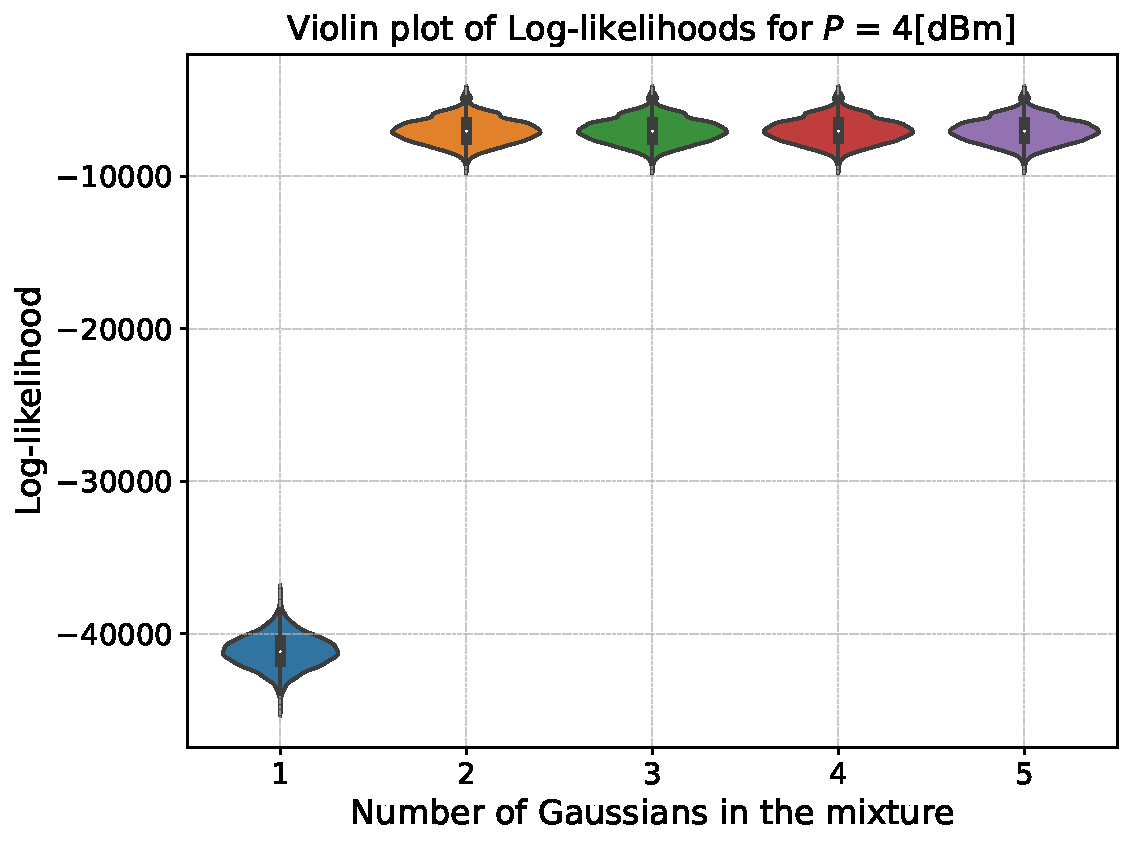
\includegraphics[width=1\linewidth]{images/gauss/bigf_loglik_pdbm_4.pdf} (d) \\
    }
    \end{minipage}

    \begin{minipage}[h]{0.5\linewidth}
    \center{
        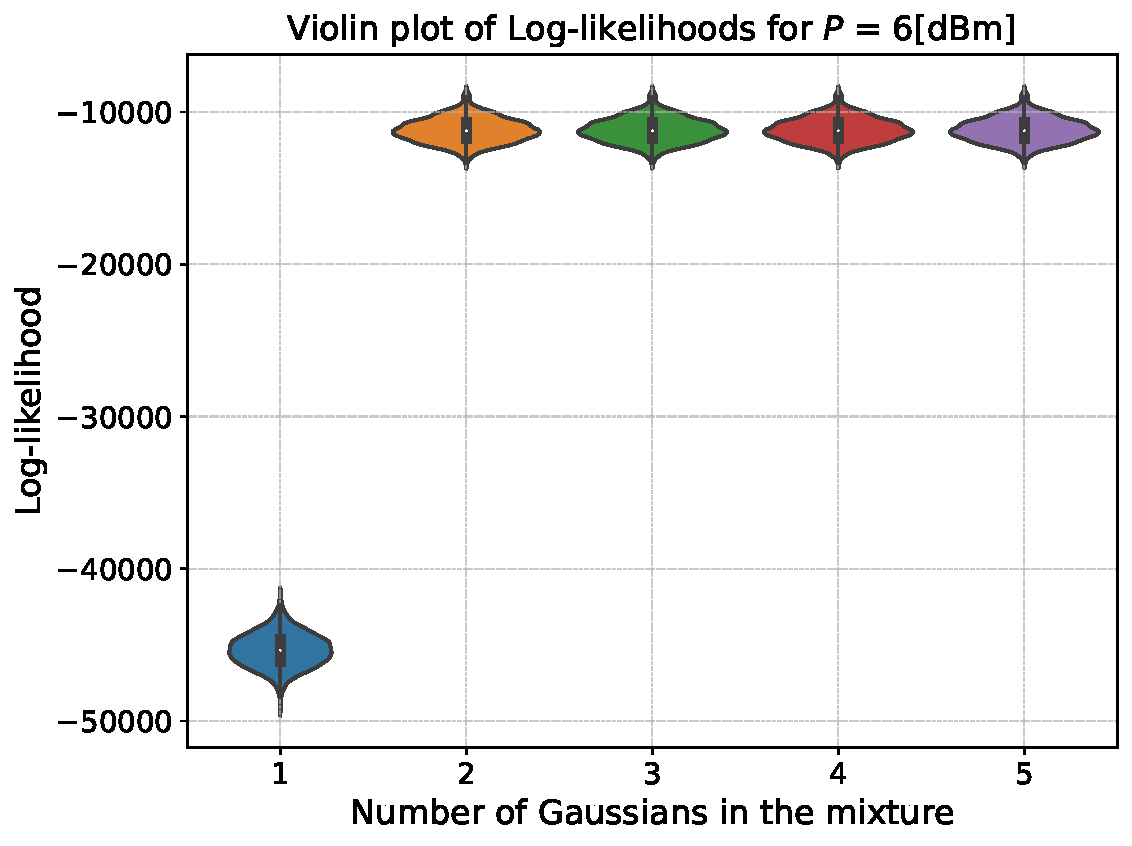
\includegraphics[width=1\linewidth]{images/gauss/bigf_loglik_pdbm_6.pdf} (e) \\
    }
    \end{minipage}
    \begin{minipage}[h]{0.5\linewidth}
    \center{
        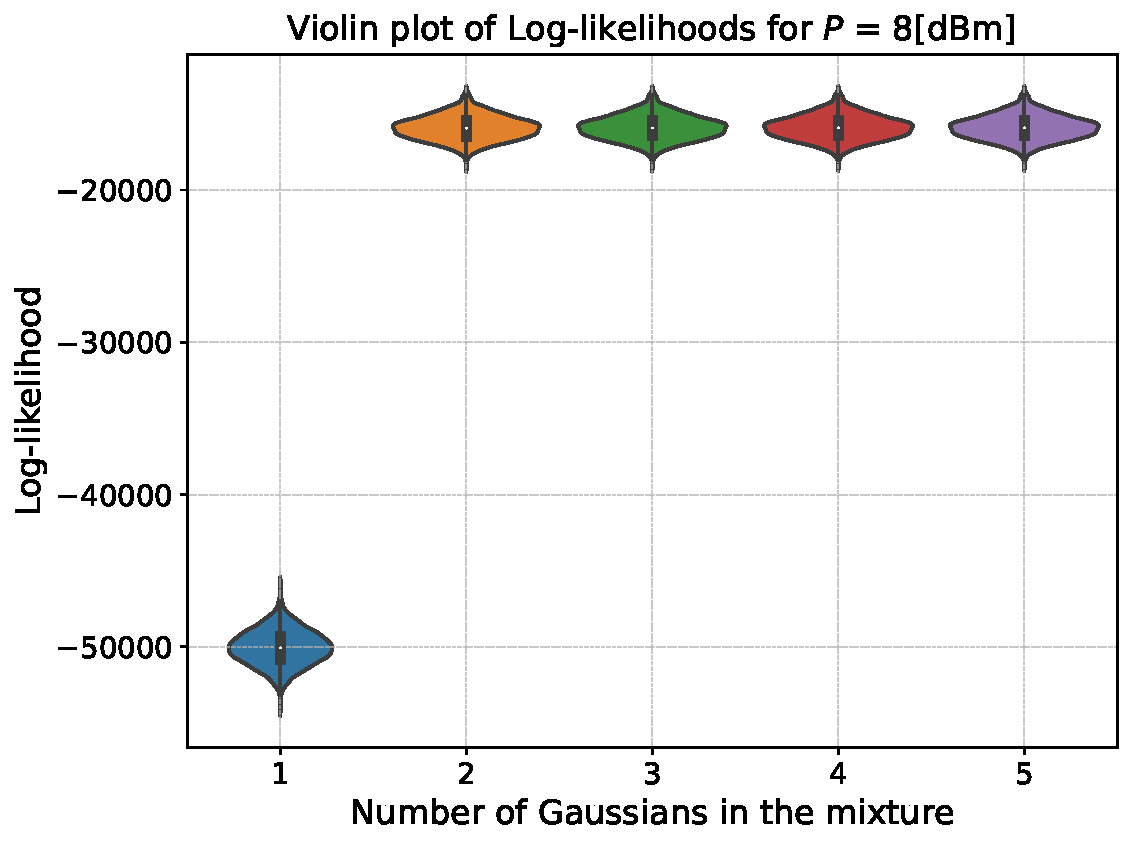
\includegraphics[width=1\linewidth]{images/gauss/bigf_loglik_pdbm_8.pdf} (f) \\
    }
    \end{minipage}

    \caption{Violin plot of log-likelihood for triplet distribution for different number of components in \gls{gmm}. \textbf{(a)} $P_{ave} = -2$ $\mathrm{[dBm]}$, \textbf{(b)} $P_{ave} = 0$ $\mathrm{[dBm]}$, \textbf{(c)} $P_{ave} = 2$ $\mathrm{[dBm]}$, \textbf{(d)} $P_{ave} = 4$ $\mathrm{[dBm]}$, \textbf{(e)} $P_{ave} = 6$ $\mathrm{[dBm]}$, \textbf{(f)} $P_{ave} = 8$ $\mathrm{[dBm]}$ }
    \label{fig:violin_different_power}
\end{figure}

Having observed that the shape of distributions for certain triplets can markedly differ when using single or multi-component \gls{gmm}, we now proceed to compare the likelihoods of these distributions. To this end, we employ the log-likelihood measure described in the previous section (see Eq.~(\ref{eq:loglik})) to test the hypothesis that our simulation distribution corresponds to a specific \gls{gmm}. Figure~\ref{fig:violin_different_mix} presents violin plots\footnote{A violin plot is a method of plotting numeric data and can be understood as a combination of a box plot and a kernel density plot. It includes a marker for the median of the data and a box indicating the interquartile range, as seen in standard box plots, overlaid with a kernel density estimation.} that illustrate the log-likelihood distribution for different average signal powers and numbers of components in the \gls{gmm}. The x-axis of each plot denotes the number of components in the \gls{gmm}, while the y-axis shows the distribution of log-likelihood values across all possible triplets. This visualization method is particularly useful given the \(2^{12}\) possible triplet combinations, which would be exceedingly challenging to depict using line plots (as demonstrated in Fig.~\ref{fig:lines_different_mix}). The average power in the graphs on Fig.~\ref{fig:violin_different_mix} ranges from -2 dBm (upper left) to 8 dBm (lower right).

Regardless of the log-likelihood values, all graphs consistently reveal that the likelihood for a single-component \gls{gmm} is significantly lower compared to a \gls{gmm} with 2, 3, 4, or 5 components, which all exhibit approximately the same log-likelihood values. This pattern holds across all levels of average signal power. However, what varies with the power is the actual value of the log-likelihood. The principal finding, however, is as follows: the likelihood that our experimental data are drawn from a single-component \gls{gmm} is exceedingly low compared to that from a multi-component \gls{gmm}. This observation aligns with our earlier discussions: a standard Gaussian distribution does not adequately fit the experimental data, necessitating the use of a more complex model comprising multiple Gaussian components.

\begin{figure}[tp]
    \begin{minipage}[h]{0.5\linewidth}
    \center{
        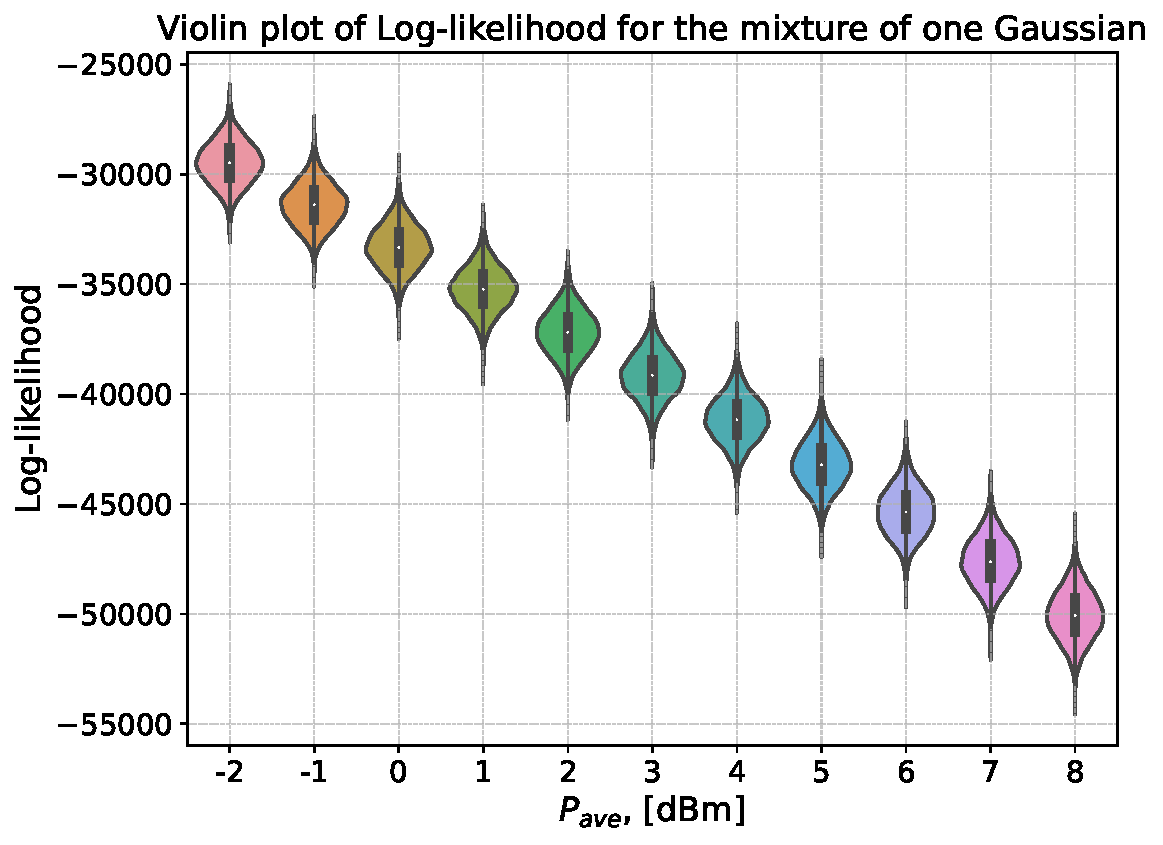
\includegraphics[width=1\linewidth]{images/gauss/bigf_h1_loglik_vs_p_ave_dbm.pdf} (a) \\
    }
    \end{minipage}
    \begin{minipage}[h]{0.5\linewidth}
    \center{
        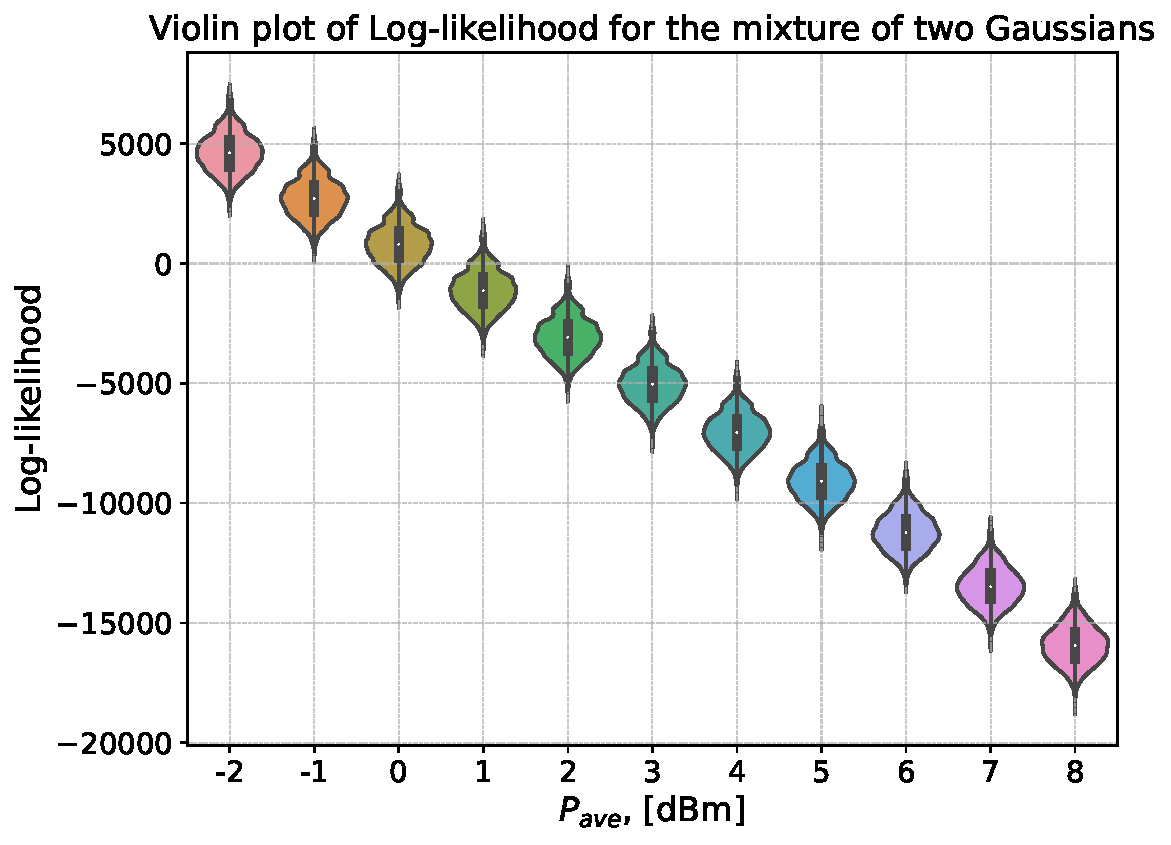
\includegraphics[width=1\linewidth]{images/gauss/bigf_h2_loglik_vs_p_ave_dbm.pdf} (b)\\
    }
    \end{minipage}

    \caption{Violin plot of log-likelihood dependence for triplet distribution on average signal power for different number of components in \gls{gmm}. One Gaussian in the mixture \textbf{(left)} and mixture of two Gaussians \textbf{(right)}.}
    \label{fig:violin_different_mix}
\end{figure}

Figure~\ref{fig:violin_different_power} presents a violin plot of the log-likelihood for triplets across various power levels, contrasting a mixture with one component (left panel) against two components (right panel). In both instances, the average log-likelihood value decreases as the power increases, suggesting the potential for more intricate structural characteristics within the distribution. Notably, even at higher power levels, the two-component \gls{gmm} provides a markedly superior fit to the experimental data; for instance, at 8 dBm, the average log-likelihood value for a single component is approximately \(-50000\), whereas for two components it is around \(-16000\). Although these values alone do not conclusively indicate that the experimental data correspond to a particular type of distribution, they do offer insights that a more suitable model might exist to describe such distributions. Furthermore, as illustrated in Fig.~\ref{fig:violin_different_power}, the decline in average log-likelihood is consistent and nearly linear with increasing average power. This observation, coupled with insights from Fig.~\ref{fig:violin_different_mix}, indicates that adding more components to the mixture does not enhance the likelihood significantly. Therefore, for our simulations, a two-component mixture is deemed sufficient for an initial approximation of data representation.

\begin{figure}[tp]
    \begin{minipage}[h]{0.5\linewidth}
    \center{
        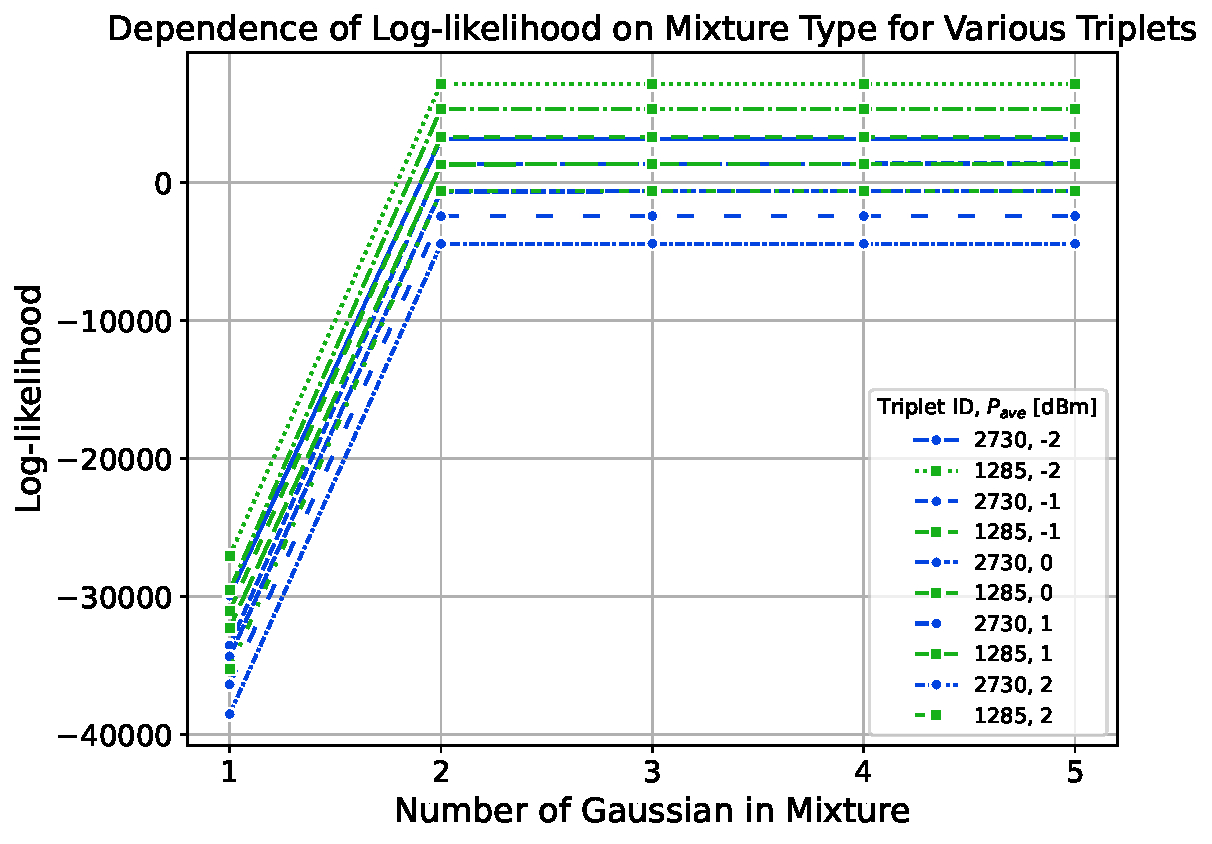
\includegraphics[width=1\linewidth]{images/gauss/bigf_loglik_vs_mixture_low.pdf} (a) \\
    }
    \end{minipage}
    \begin{minipage}[h]{0.5\linewidth}
    \center{
        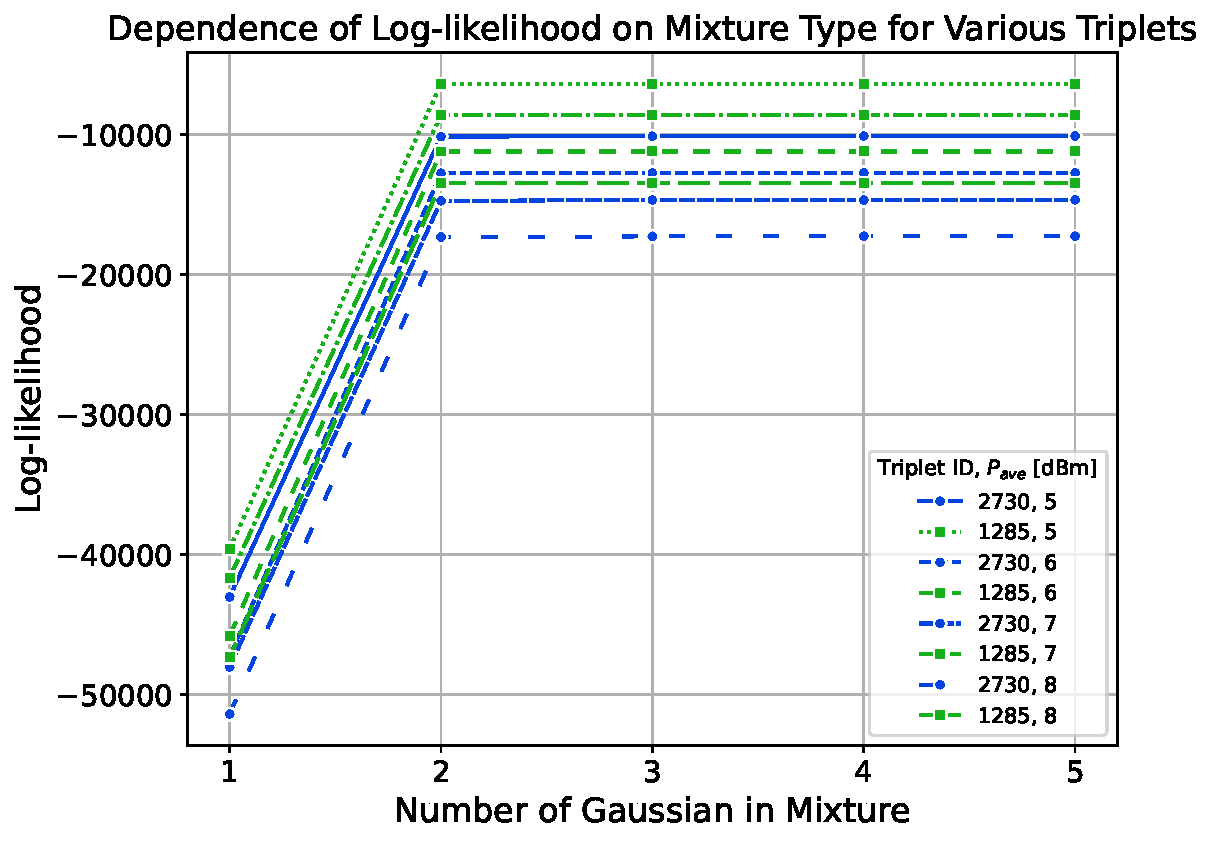
\includegraphics[width=1\linewidth]{images/gauss/bigf_loglik_vs_mixture_high.pdf} (b)\\
    }
    \end{minipage}

    \caption{Log-likelihood dependence for triplet distribution for different number of components in \gls{gmm}. Graph shows triplets with ID 2730 $[3+3\mathrm{i}, 3+3\mathrm{i}, 3+3\mathrm{i}]$ and ID 1285 $[-1-1\mathrm{i}, 1+1\mathrm{i}, -1-1\mathrm{i})]$.}
    \label{fig:lines_different_mix}
\end{figure}

Figures~\ref{fig:lines_different_mix} and~\ref{fig:loglik_for_triplets} offer a different view of the same data depicted by the violin plots in Figures~\ref{fig:violin_different_mix} and~\ref{fig:violin_different_power}, focusing on specific triplets. This perspective is valuable because violin plots can obscure the behavior of log-likelihood for individual triplets. These figures confirm a consistent finding: there is a substantial difference in the log-likelihood values between the single Gaussian model and a mixture of several Gaussians. The log-likelihood stabilizes with an increasing number of components in the \gls{gmm}, indicating that a mixture of two Gaussians is typically adequate. The same trend is observed with the log-likelihood's response to signal power: it decreases linearly as the average power increases. Additionally, for a \gls{gmm} with two components, the lines representing different triplets do not cross, affirming the consistency of this pattern.


\begin{figure}[htpb]
    \center{
        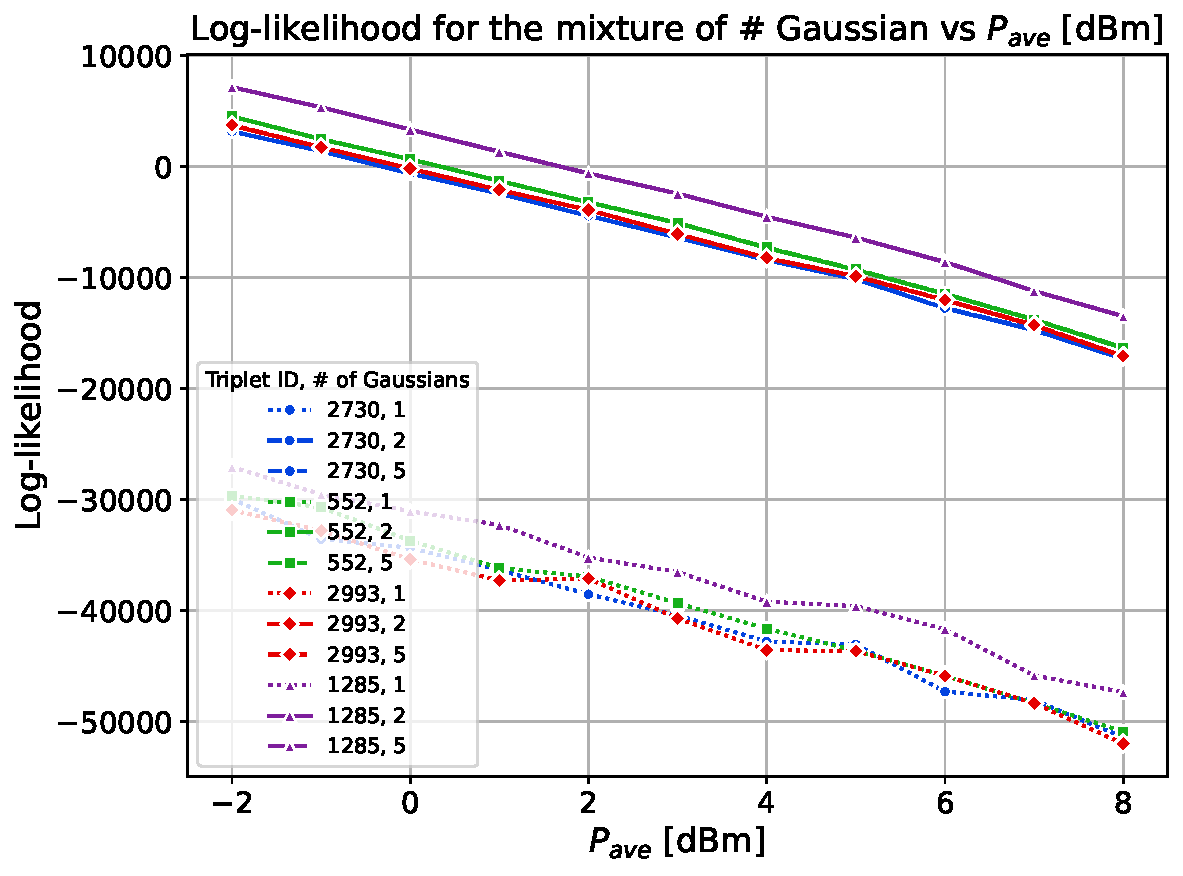
\includegraphics[width=0.7\linewidth]{images/gauss/bigf_loglik_for_triplet.pdf} \\
    }
    \caption{Dependence of log-likelihood for triplet distribution on average signal power for different number of components in \gls{gmm}. Graph shows triplets with ID 2730 $[3+3\mathrm{i}, 3+3\mathrm{i}, 3+3\mathrm{i}]$, ID 1285 $[-1-1\mathrm{i}, 1+1\mathrm{i}, -1-1\mathrm{i}]$, ID 2993 $[3-3\mathrm{i}, 3-3\mathrm{i}, 1-1\mathrm{i}]$ and ID 552 $[1+3\mathrm{i}, 1+3\mathrm{i}, 3+1\mathrm{i}]$.}
    \label{fig:loglik_for_triplets}
\end{figure}

\section{Discussion}
In digital communications understanding the impact of nonlinear effects is crucial for improving signal integrity and system performance. This research delves into the analysis of these effects through the lens of \acrlong{gmm}, focusing on a constrained set of data points -- triplets -- to manage computational complexity and provide meaningful insights into the behavior of the system under nonlinear influences.

\subsection{Computational Feasibility}
Given the constraints of high-speed data generation tools, both time and storage space are limiting factors in our research. The choice to analyze triplets, resulting in $2^{12}$ possible combinations from a 16-\acrshort{qam} constellation, allows for a manageable dataset of $2^{24}$ data points, ensuring an average of $2^{12}$ points per combination for robust analysis. Expanding the neighborhood analysis to include pairs, thereby increasing the combinations to $2^{20}$, would necessitate $2^{32}$ data points -- a 256-fold increase -- rendering the analysis impractical with current resources. For instance, fitting a \acrshort{gmm} to one power level of 4096 triplets took approximately two hours on a standard workstation; extending this to five-point combinations would extend the analysis time to an impractical duration, approximately one month for a single power level, highlighting a significant gap in computational efficiency that is beyond the scope of this study.

\subsection{Approach}
The study of neighbor influences within signal transmission represents an iterative evolution in understanding how information is transformed and perceived. Initially, the focus was on the direct transformation of a transmitted point through signal propagation to its received counterpart, leading to rigid decision boundaries devoid of contextual data. Subsequently, the exploration expanded to include neighboring symbols at the receiver, aiming to enhance equalization accuracy through this supplementary information. For instance, as discussed in Section~\ref{sec:gradient_boosting}, the gradient boosting approach leverages data about received points and their neighbors to infer the original transmitted point.

Progressing beyond this, our research introduces an alternative perspective by examining the impact of sending sequence neighbors (rather than those received) on the configuration of received points. This method does not specify the propagation distance; instead, it investigates how neighboring points from the transmitter influence the received signal. The core objective of this work is to demonstrate how varying combinations of triplets lead to unique structures in the received points, driven by nonlinear effects. This phenomenon is attributed to the complex interplay within the nonlinear system, where the subsequent neighbors' influence is also embedded in the resulting distribution. By increasing the dataset size, we can generalize the effect of different sequences of subsequent neighbors, providing a clearer understanding of the distribution patterns that emerge. This approach not only deepens our comprehension of signal propagation dynamics but also lays the groundwork for future enhancements in signal processing techniques.

\subsection{Future Directions}
In this phase of our analysis, the focus is intentionally not placed on the neighbors at the receiver, as the primary objective is to lay the groundwork for developing a message passing (MP) algorithm. This algorithm is envisaged to adopt a comprehensive approach by incorporating information about neighboring points, thereby facilitating more informed decision-making regarding the received points based on the sequence of neighbors. The algorithm will dynamically determine the optimal number of neighbors to consider, a parameter that will be fine-tuned in future studies to enhance performance. Utilizing the distribution information for triplets, the MP algorithm aims to refine solution accuracy. While the potential exists to extend this analysis to more complex structures involving five or more points, the current focus on triplets and their probability distributions is deemed sufficient for significantly improving decoding performance. Consequently, there is no immediate requirement to analyze longer initial sequences; this research marks a preliminary step towards the development of a sophisticated algorithm.

\subsection{Conclusion}
In summary, this research marks a pioneering step towards understanding how nonlinearities influence signal structures in 16-\acrshort{qam} systems, revealing that these structures deviate significantly from Gaussian models. Our investigation underscores the complexity inherent in the distribution of received signals, where \acrlong{gmm} enhance fit but reach a saturation point in effectiveness with additional components. While the validation of these findings through error rate calculations has not been undertaken within the scope of this thesis, it forms a critical component of our ongoing research agenda.

Future directions will explore beyond the \acrshort{gmm} to discover if alternative or more intricate models could more accurately capture the nuances of signal distributions. The immediate next step involves developing an algorithm that utilizes the \acrshort{gmm} framework to predict the distribution category of received signals. By calculating the likelihood across different models, we can identify the most fitting distribution for a given signal point. Integrating message passing algorithms could further refine this prediction process, offering a robust tool for decoding signal distributions. Preliminary work is already underway, with the aim of substantiating the practical benefits of the proposed \acrshort{gmm} configuration through rigorous error rate analysis in future publications.

Moreover, the analytical insights into signal distribution patterns hold promise for channel monitoring applications. Notably, discrepancies from anticipated distributions may signal underlying system issues, providing a novel diagnostic approach to maintain the operational integrity of optical communication networks.

Expanding this analysis to encompass various modulation formats and system configurations represents an exciting avenue for further research. The use of the HpCom~\cite{esf0_2023_7880552} package will be instrumental in generating relevant statistics, facilitating a broad-based exploration of optical communication systems.
Embracing these avenues for future investigation will not only deepen our understanding of the dynamics within optical communication systems but also contribute to enhancing their efficiency and reliability.



% \section{Conclusion}
% In summarizing the findings from our analysis, we have identified that while the \Gls{gmm} provides an improved fit over a single Gaussian model for the received signal distributions in a 16-QAM WDM optical communication system, the likelihood does not increase with additional Gaussian components. This suggests a saturation point in the utility of adding complexity to the GMM for this system. Consequently, future work should consider exploring more complex distributions beyond GMMs to ascertain if other types or combinations may yield a more accurate representation of the experimental data.

% For practical applications, the next steps include the development of an algorithm that leverages GMM to predict which distribution a received point corresponds to. By evaluating the likelihood for different distributions, we can ascertain the most probable model for a given signal point. Advanced techniques, such as message passing algorithms, may enhance this predictive capability.

% Furthermore, the insights gained from analyzing the distribution of received points could inform channel monitoring strategies. Significant deviations from the expected distribution pattern might indicate systemic issues, offering a diagnostic tool to ensure the integrity of optical communication systems.

% Extending this analysis to other modulation formats and system types is a viable direction for further research. Utilizing the HpCom package can facilitate the creation of corresponding statistics, enabling a comprehensive investigation across various system configurations.

% By adopting this focused approach to further analysis, we can expand our understanding of optical communication systems and improve their performance and reliability.